\documentclass[fleqn, final]{../styles/unmphythesis}
\usepackage{../styles/qxd}
\renewcommand{\thechapter}{4}
%\newcommand{\thechapter}{1}

\makeindex
\begin{document}

%<*quantumdynamics>

\chapter[QND measurement and spin squeezing using photonic waveguides]{Quantum non-demolition measurement and spin squeezing using nanophotonic waveguides}\label{chap:quantumdynamicsrepresentation}
\section{Introduction}
So far, we have treated the light as a classical field. 
In this chapter, we will fully quantize the optical field and study the quantum noise origin of the light by redefining the Stokes operators using the bosonic operators, and introduce the Hamiltonian of the atom-light interaction for the quantum non-demolition (QND) measurement. We will also link the collective spin operators to the traditional squeezing operators and finally introduce the QND-measurement--induced spin squeezing. 

\section[Atom-light coupling with waveguide modes]{Atom-light coupling with waveguide modes}
We consider atoms trapped on a one- or two-side chain of optical lattice near a nanophotonic waveguide. A probe is launched to perform the quantum measurement using the polarization spectroscopy technique introduced in the Chapter~\ref{chap:waveguideinterfaces}. We assume all atoms are trapped the same distance to the waveguide surface with the same local intensity of the probe. Defects of occupations on the optical lattices are allowed in our theory, and the minimum distance between the atoms is large enough that we can ignore the photon scattering effect among atoms in the dispersive regime. 
We concentrate on the waveguides that allow two orthogonally polarized forward-propagating guided modes with degenerate group index of refraction, $ n_g $. 

%Experiments on implementing such an atom-waveguide quantum interface have been done with optical nanofibers~\cite{Goban2012,Lacroute2012,Vetsch2010Optical,Lee2015,Beguin2014,Bajcsy2011Laser}, integrated optical waveguide couplers~\cite{Lee2013} and photonic crystal waveguides~\cite{Yu2014,Goban2014}. The designs of general nanophotonic waveguides for feasible atomic traps and atom-light interaction experiments have also been proposed for a broader range of atom-waveguide interfaces~\cite{Muniz2015Designing,Hung2013,Lee2017Characterizations}. 

Given an input light that adiabatically connects to the forward-propagating quasi-monochromatic $ p $-mode at frequency $ \omega_0 $, we define the field operators $ \hat{a}^\dagger_p(z,t) $ by~\cite{Gardiner1985Input,Blow1990Continuum,LeKien2008}
	\begin{align}
		\hat{a}_{p}(z,t) =\frac{1}{\sqrt{2 \pi}}  \int_0^{\infty}\!\!\!\!\! d \omega \, \hat{a}_{p}(\omega) e^{i[\beta_0 z- (\omega-\omega_0) t ]}, 
	\end{align}
that satisfy the free-field commutation relations,
	\begin{equation} \label{Eq::InputOutputCommutation_a}
		\big[\hat{a}_{p}(z,t),\hat{a}^\dag_{p'}(z',t')\big]=\delta_{p,p'}  \delta(t-t'-(z-z')/v_g).
	\end{equation}
The corresponding positive-frequency electric field operators in the orthogonal mode basis can be defined as
	\begin{equation} \label{Eq::PropagatingElectricField_forward}
		\hat{\mathbf{E}}^{(+)}(r\!_\perp,\phi,z;t) = \sum_{p} \sqrt{ \frac{2 \pi \hbar \omega_0}{ v_g} } \mathbf{u}_{p}(r\!_\perp,\phi) \hat{a}_{p}(z,t)  e^{i \beta_0 z},
	\end{equation}	
where the sum over $ p $ includes all components of a complete mode basis. Below, we only consider the $ \{H,V \} $ mode basis. The transformation of operators to another arbitrary mode bases is derived in Appendix~\ref{chap:basistransfHS}. 

With $ N_A $ atoms interacting with the propagating electric field of the local guided modes, the dispersive light-shift Hamiltonian can be defined as~\cite{Deutsch2010a,LeKien2013,Baragiola2014Open},
	\begin{equation} \label{Eq::LightShiftHam_forward}
		\hat{H}_{LS} = \sum_{n=1}^{N_A} \hat{h}_{\rm eff},
	\end{equation}
with the light-atom interaction Hamiltonian with one atom given by
\begin{align}
\hat{h}_\eff &= -\hat{\mathbf{E}}^{(-)}(\br')\cdot\hat{\tensor{\boldsymbol{\alpha}}}\cdot\hat{\mathbf{E}}^{(+)}(\br')\label{eq:HEalphaE}\\
&= -\frac{2\pi\hbar\omega}{v_g}\left[\mathbf{u}_H^*\cdot\hat{\tensor{\boldsymbol{\alpha}}}\cdot \mathbf{u}_H\hat{a}_H^\dagger\hat{a}_H\right.
+ \mathbf{u}_H^*\cdot\hat{\tensor{\boldsymbol{\alpha}}}\cdot \mathbf{u}_V\hat{a}_H^\dagger\hat{a}_V\nn\\
&\quad\quad + \mathbf{u}_V^*\cdot\hat{\tensor{\boldsymbol{\alpha}}}\cdot \mathbf{u}_H\hat{a}_V^\dagger\hat{a}_H 
\left. + \mathbf{u}_V^*\cdot\hat{\tensor{\boldsymbol{\alpha}}}\cdot \mathbf{u}_V\hat{a}_V^\dagger\hat{a}_V\right] \label{eq:heff_uhvalpha}\\
&= \hbar\left[(\hat{\chi}_{HH}+\hat{\chi}_{VV})\hat{S}_0 + (\hat{\chi}_{HH}-\hat{\chi}_{VV})\hat{S}_1 \right.\nn\\
&\quad \quad\left. + (\hat{\chi}_{HV}+\hat{\chi}_{VH})\hat{S}_2 + i(\hat{\chi}_{HV}-\hat{\chi}_{VH})\hat{S}_3 \right]\\
%\hbar \left[\left(\chi_{RR\uparrow} + \chi_{RR\downarrow} +\chi_{LL\uparrow}+\chi_{LL\downarrow} \right)\hat{F}_0\hat{S}_0 \right.\nonumber\\
%&\quad+\left(\chi_{RR\uparrow} + \chi_{RR\downarrow} -\chi_{LL\uparrow}-\chi_{LL\downarrow} \right)\hat{F}_0\hat{S}_3\nonumber\\
%&\quad+\left(\chi_{RR\uparrow} + \chi_{LL\uparrow} -\chi_{RR\downarrow}-\chi_{LL\downarrow} \right)\hat{F}_3\hat{S}_0\nonumber\\
%&\quad+\left(\chi_{RR\uparrow} - \chi_{RR\downarrow} +\chi_{LL\downarrow}-\chi_{LL\uparrow} \right)\hat{F}_3\hat{S}_3\nonumber\\
%&\quad+i\left(\chi_{LR\uparrow} - \chi_{RL\uparrow} +\chi_{RL\downarrow}-\chi_{RL\downarrow} \right)\hat{F}_0\hat{S}_1\nonumber\\
%&\quad+\left(\chi_{RL\uparrow} + \chi_{LR\uparrow} +\chi_{RL\downarrow}+\chi_{LR\downarrow} \right)\hat{F}_0\hat{S}_2\nonumber\\
%&\quad+i\left(\chi_{LR\uparrow} - \chi_{RL\uparrow} +\chi_{RL\downarrow}-\chi_{LR\downarrow} \right)\hat{F}_3\hat{S}_1\nonumber\\
%&\quad+\left.\left(\chi_{LR\uparrow} + \chi_{RL\uparrow} -\chi_{LR\downarrow}-\chi_{RL\downarrow} \right)\hat{F}_3\hat{S}_2 \right]\\
&=\hbar\sum_{i=0}^3 \hat{\chi}_{i}\hat{S}_i \label{eq:heff_chifS}
%&=\hbar\sum_{i,j=0} \chi_{ij}\hat{f}_i\hat{S}_j,
\end{align}
where $\poltens$ is the atomic tensor polarizability operator, given in \erf{Eq::AtomicPolarizabilityF}, for each atom trapped near the waveguide surface at position $\mathbf{r}'_\perp$ in the transverse plane. Here, we ignore any effects of atomic motion and treat the atoms as localized at fixed positions in space. We have also defined $ \hat{S}_i $ as the Stokes vector operators of the light indicating its polarization, which are the quantum counterparts of the classical definition in Eq.~\eqref{eq:S_xybasis}. The vector Stokes operators that describe the polarization of the propagating fields in the quasilinear $HV$-basis are given as below:
\begin{subequations}\label{Eq::StokesComponents_general}
	\begin{align} 
		\hat{S}_1(t) & = \smallfrac{1}{2}\big[ \hat{a}^\dag_H(t) \hat{a}_H(t)-\hat{a}^\dag_V(t) \hat{a}_V(t) \big], \\
	 	\hat{S}_2(t) & = \smallfrac{1}{2}\big[ \hat{a}^\dag_H(t) \hat{a}_V(t)+\hat{a}^\dag_V(t) \hat{a}_H(t) \big], \\ 
		\hat{S}_3(t) & = \smallfrac{1}{2i}\big[ \hat{a}^\dag_H(t) \hat{a}_V(t) -\hat{a}^\dag_V(t) \hat{a}_H(t) \big],
	\end{align}
\end{subequations}
that satisfy equal-$z$ commutation relations following from \erf{Eq::InputOutputCommutation_a},
	\begin{equation} \label{Eq::StokesCommutation}
		\big[\hat{S}_i(t), \hat{S}_j(t')\big] =i \epsilon_{ijk} \delta(t-t')  \hat{S}_k(t).
	\end{equation}
These, along with the total photon flux operator,
	\begin{equation}
		\hat{S}_0(t) = \smallfrac{1}{2}\big[ \hat{a}^\dag_H(t) \hat{a}_H(t)+\hat{a}^\dag_V(t) \hat{a}_V(t) \big],
	\end{equation}
are the quantum version of the Stokes vectors defined in Eq.~\eqref{eq:S_intensitydiff}. 
We also define the mode-atom coupling operator
\begin{align}
\hat{\chi}_{pp'} 
&=-\frac{2\pi \omega}{v_g}\mathbf{u}_{p}^*(r'\!_\perp,\phi')\cdot \hat{\tensor{\alpha}}\cdot \mathbf{u}_{p'}(r'\!_\perp,\phi')\\
&= \sum_{f'} \frac{n_g\sigma_0}{4}\frac{\Gamma_{f'}}{\Delta_{ff'}+i\Gamma_{f'}/2}\cdot \left\{ C_{j'ff'}^{(0)}\mathbf{u}_p^*(r'\!_\perp)\cdot \mathbf{u}_{p'}(r'\!_\perp)\hat{\mathbbm{1}}\right.\nn\\
&\quad\quad +iC_{j'ff'}^{(1)}\left(\mathbf{u}_p^*(r'\!_\perp)\times\mathbf{u}_{p'}(r'\!_\perp) \right)\cdot \hat{\mathbf{f}} \nonumber\\
&\quad\quad\left. + C_{j'ff'}^{(2)}\sum_{i,j}\left[u^*_{p,i}u_{p',j}(\frac{\hat{f}_i\hat{f}_j+\hat{f}_j\hat{f}_i}{2}-\frac{\delta_{ij}}{3}\hat{\mathbf{f}}\cdot\hat{\mathbf{f}}) \right]\right\}
%&\left.+C_{jj'ff'}^{(2)}\left[\mathbf{u}_p^*(r'\!_\perp)\cdot \mathbf{u}_{p'}(r'\!_\perp)\left(\frac{f(f+1)}{6}-\frac{m^2}{2} \right)+\mathbf{u}_p^*(r'\!_\perp)\cdot (\hat{e}^*_{\tilde{z}}\hat{e}_{\tilde{z}})\cdot \mathbf{u}_{p'}(r'\!_\perp)\left(\frac{3m^2}{2}-\frac{f(f+1)}{2} \right) \right] \right\}
\label{eq:chippp}
\end{align}
with the horizontally(H)- and vertically(V)-linearly polarized guided modes, $ \mathbf{u}_p(r'\!_\perp) $, at the atom position $ \br'=(r'\!_\perp,\phi',z') $. 
$ \hat{\mathbf{f}} $ is the total atomic angular moment operator.
%$ \chi_{ij}=\tr[\hat{f}_i\hat{\chi}_j]/(2f+1) $ is the coupling strength between spin operator $ \hat{f}_i $ and Stokes operator $ \hat{S}_j $. 
%For example, $ \chi_{33} $ is the coupling strength between $ \hat{f}_z $ and $ \hat{S}_3 $.
The coupling operator or Eq.\eqref{eq:chippp} includes three terms corresponding to scalar, vector and tensor interactions between atoms and the probe light which are proportional to $ C_{j'ff'}^{(K)} $ with $ K=0,\,1,\,2 $, respectively.
These terms may vanish depending on the state of atoms and the polarization state of the probe defined for the atom-light interaction protocol.

Consequently, by writing the polarizability tensor in the irreducible representation [Eq.~\eqref{Eq::IrreducibleDecomp}], we can also write the Hamiltonian in the following form~\cite{Deutsch2010a}:
\begin{align}  
\hat{h}_{\rm eff} &= - \sum_{f,f'}\alpha_0(\Delta_{f,f'}) \left\{ C_{j'ff}^{(0)} \hat{\mathbf{E}}^{(-)} \cdot \hat{\mathbf{E}}^{(+)} \hat{\mathbbm{1}}_f \phantom{\frac{\hat{1}}{1}}\right. \nonumber\\
&\quad\quad\quad + i C_{j'ff'}^{(1)} \left(\hat{\mathbf{E}}^{(-)} \times \hat{\mathbf{E}}^{(+)} \right) \cdot \hat{ \mathbf{f}} \nonumber\\
&\quad\quad\quad  \left. + C_{j'ff}^{(2)} \hat{E}_i^{(-)} \hat{E}_j^{(+)} \left( \frac{ \hat{f}_i \hat{f}_j  + \hat{f}_j \hat{f}_i  }{2} - \frac{1}{3}\delta_{ij} \hat{ \mathbf{f}} \cdot \hat{\mathbf{f}}  \right) \right\}. \label{Eq::LightShiftHam_irep}
\end{align} 
Every line above corresponds to the scalar, vector and tensor light shift Hamiltonian. 

\section{Some special states of alkali atoms}
In this section, we highlight two sets of states of alkali atoms, particularly, $ ^{133} $Cs atoms: one is the \emph{clock states}\index{state!clock state}, and the other one is the \emph{stretched states}\index{state!stretched state}. We will use these states and coupled state subspace to design QND measurement and induced spin squeezing protocols in later chapters. 

Beside the states of individual atoms, we will also introduce some interesting collective states in this section. 

\subsection{Clock states and clock space}
%There are two hyperfine levels with $ f=3 $ and $ f=4 $ on the ground state, $ 6S_{1/2} $, of $ ^{133} $Cs atoms. 
%The hyperfine ground splitting is approximate $9.2$ GHz. Optical pumping can be implemented with fine structure transitions from $6S_{1/2} \rightarrow 6P_{1/2}$ (D1 line transitions) or from $6S_{1/2} \rightarrow 6P_{3/2}$ (D2 line transitions), 
%which are separated by tens of THz and thus quite resolvable.   

%Now suppose that rather than using the magnetic sublevels within a single ground hyperfine state $f$, 
We begin with a dispersive interface defined on the $m=0$ \emph{clock states}\index{state!clock state} between the $f=3$ and $f=4$ hyperfine states of $ 6S_{1/2} $.  To first order, such states are insensitive to ambient 
magnetic field fluctuations, which make the clock state space useful for implementing atomic clocks.  In the clock-state subspace, we designate the qubit states
\begin{align} 
	\ket{\uparrow} &\equiv \ket{f = 4,m = 0}, \\
 	\ket{\downarrow} &\equiv \ket{f = 3,m=0},
\end{align}
where $ m $ are the quantum numbers of the projected $ f $ manifold sublevels (see Fig.~\ref{fig:D1line_F3F4}).
If we define a subspace in the $ x $ basis that 
\begin{align}
\ket{\uparrow_x} = \frac{1}{\sqrt{2}}(\ket{\uparrow}+\ket{\downarrow}),\\
\ket{\downarrow_x} = \frac{1}{\sqrt{2}}(\ket{\uparrow}-\ket{\downarrow}),
\end{align}
and the corresponding Pauli-$ z $ operator 
\begin{align}
\hat{\sigma}_z = \ket{\uparrow_x}\bra{\downarrow_x}+ \ket{\downarrow_x}\bra{\uparrow_x},
\end{align}
we have $ \hat{\sigma}_z\ket{\uparrow_x}=\ket{\downarrow_x} $ and $ \sigma_z\ket{\downarrow_x}=\ket{\uparrow_x} $. 
Therefore, the clock states $ \{\ket{\uparrow},\ket{\downarrow} \} $ form a closed subspace for the Pauli-$ z $ transitions. 
Since this subspace is a pseudo spin-$ 1/2 $ space, we use the spin-$ 1/2 $ operator, $ \hat{\mathbf{j}}=\hat{\boldsymbol{\sigma}}/2 $, to denote the total atomic angular moment, with the Pauli operator $ \hat{\boldsymbol{\sigma}} $ defining the spin state transformations.
For $ N_A $ atoms, the collective spin operator, 
\begin{align}
\hat{\mathbf{J}} = \sum_n^{N_A} \hat{\mathbf{j}}^{(n)}
\end{align}
defines the collective measurement operators, where $ \hat{\mathbf{j}}^{(n)} $ is the spin operator for the $ n $th atom. 
%Note that, in discussing the QND measurement protocols in Chapter~\ref{chap:birefringence}, we define operators in the $ z $ basis instead, and $ \hat{J}_z $ becomes the spin squeezing operator. But the physics is the same.

%Not to go into too much details, below, we briefly review two approaches to simplify the light-shift Hamiltonian using the Clebsch-Gordan coefficients and the irreducible tensor representation, respectively. Some basic properties of the clock space will also be discussed.
\begin{figure}[!tbp]
\centering\makebox[\textwidth]{
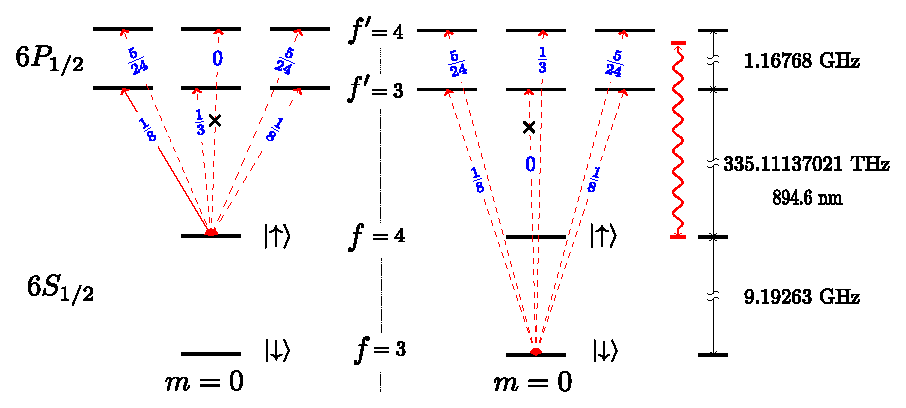
\includegraphics[width=0.8\textwidth]{../media/Figs/D1line_F3F4}}
\caption[D1 line transitions in the clock space.]{D1 line transitions in the clock space. The red dashed lines show quantum transitions connected to an excited state on the $ 6P_{1/2} $ levels and a ground state on the $ 6S_{1/2} $ levels (probabilities on the lines) of the $ \ket{\uparrow}=\ket{f=4,m=0} $ clock state (left) and the $\ket{\downarrow}=\ket{f=3,m=0}$ clock state (right). 
Transitions between $ \ket{\uparrow} $ and $ \ket{f'=4,m=0} $, and between $ \ket{\downarrow} $ and $ \ket{f'=3,m=0} $ are forbidden. $ \sigma_\pm $ transitions are symmetric for both clock states and connect the two clock states. }\label{fig:D1line_F3F4}
\end{figure}

We consider the case that the atoms are placed at points on the $ x $ axis and a $ D $ mode of light is propagating through the waveguide. There are two useful properties of the system with atoms in the clock space.

First, the cross couplings between $ H $ and $ V $ modes vanish in \erf{eq:heff_uhvalpha}. We give an outline of the proof below.
%In the clock state subspace, the light shift Hamiltonian, \erf{eq:heff_uhvalpha}, can be expressed in these state basis by finding 
%the 
%matrix elements between two relevant states.  
Since the atomic polarizability tensor is block-diagonal grouped by the level energies in 
the ground hyperfine states, we need only to consider coupling between the states within the same manifold.  
For instance, we may have a $H-V$ mode cross term like
\begin{align} \label{eq:ClockMatrixElement}
	&\bra{f,0} \mathbf{u}^*_H(r^\prime\!_\perp, \phi') \cdot \poltens \cdot 
	\mathbf{u}_{V}(r^\prime\!_\perp, \phi') \ket{f,0}\nonumber\\
  =& \!
	\sum_{f'} \sum_{m'} \sum_{q, q'}\!\! \alpha_0(f\!,f') \big( \mathbf{e}_q \!\cdot\! 
	\mathbf{u}^*_H(r^\prime\!_\perp, \phi') \big) 
	\big( \mathbf{e}^*_{q'} \!\cdot\! \mathbf{u}_V(r^\prime\!_\perp, \phi') \big) |o^{j'f'}_{jf} |^2 C^{f 0;1 
	q}_{f' m'} C^{f 
	0;1q'}_{f' m'} \\
 = & \sum_{f'} \sum_{q} \alpha_0(f,f') \big( \mathbf{e}_q \cdot \mathbf{u}^*_H(r^\prime\!_\perp, \phi') 
	\big) \big( 
	\mathbf{e}^*_{q} \cdot \mathbf{u}_V(r^\prime\!_\perp, \phi') \big) |o^{j'f'}_{jf} |^2 C^{f 0;1q}_{f' q} 
	C^{f 0;1q}_{f' q}.
\end{align}
We have used $q+q' = 0$ and for the clock states $m' = q'$. By the nature of the nanofiber modes, if we choose the
$V$-mode polarization axis or the $y$ axis to be the quantization axis, then with the atoms positioned 
along the $x$ axis, the cross term above always cancels. The same conclusion goes to other mode cross 
terms in the Hamiltonian. In fact, this result does not depend on the choice of basis. We can show that by 
rewriting the cross term above as
\begin{align}
&\bra{f,0} \mathbf{u}^*_H(r^\prime\!_\perp, \phi') \cdot \poltens \cdot 
	\mathbf{u}_{V}(r^\prime\!_\perp, \phi') \ket{f,0}\nonumber\\
=& \mathbf{u}^*_H(r^\prime\!_\perp, 
 \phi')\cdot \left[  \sum_{q} \sum_{f'}\alpha_0(f,f') 
   |o^{j'f'}_{jf} |^2 C^{f 	0;1q}_{f' q} C^{f 0;1q}_{f' q}
     	  \mathbf{e}_q \mathbf{e}^*_{q}  \right]\cdot \mathbf{u}_V(r^\prime\!_\perp, \phi') \\
=& \mathbf{u}^*_H(r^\prime\!_\perp,  \phi')\cdot \tensor{\boldsymbol{\alpha}}^{f0;f0}]\cdot 
\mathbf{u}_V(r^\prime\!_\perp, \phi') \\
=& \tr\left[ \left(  \mathbf{u}_V(r^\prime\!_\perp, \phi')  \mathbf{u}^*_H(r^\prime\!_\perp,  \phi')\right)
\cdot  \tensor{\boldsymbol{\alpha}}^{f0;f0} \right]\\
=& \frac{1}{2\pi k_0 n_g} \tr\left\{\im \left[\GFT_{VH}(\br',\br') \right] \cdot \tensor{\boldsymbol{\alpha}}^{f0;f0} \right\},
\end{align}
where 
\begin{align} 
\!\!\!\! \GFT_{VH}(\br',\br') &= i2\pi k_0 n_g 
\mathbf{u}_{V}(r^\prime\!_\perp,\phi')\mathbf{u}_{H}^*(r^\prime\!_\perp,\phi'),\\
\tensor{\boldsymbol{\alpha}}^{f0;f0} &= \bra{f,0}\boldsymbol{\alpha}\ket{f,0} = \sum_{q} 
\sum_{f'}\alpha_0(f,f') 
   |o^{j'f'}_{jf} |^2 C^{f 	0;1q}_{f' q} C^{f 0;1q}_{f' q}
     	  \mathbf{e}_q \mathbf{e}^*_{q}.
\end{align}
Obviously, rewritten as a trace, the result above does not depend on how we choose the basis. 
Using this property, the Hamiltonian, Eq.~\eqref{eq:heff_uhvalpha}, restricted in the $ \{\ket{\uparrow},\ket{\downarrow} \} $ clock spate can be rewritten as the following form without cross terms of modes:
% by 
%$\tr\left[ \mathbf{P} \left(  \mathbf{u}_V(r^\prime\!_\perp, \phi')  \mathbf{u}^*_H(r^\prime\!_\perp,  
%\phi')\right) \mathbf{P}^{-1}
%\cdot \mathbf{P}  \boldsymbol{\alpha}^{F0;F0}\mathbf{P}^{-1} \right]  $, where $ \mathbf{P} $ is the 
%rotation matrix.  
\begin{align}
\hat{h}_{\rm eff} & =  \hbar \Big( \chi_{H,\uparrow}\op{\uparrow}{\uparrow} +  
\chi_{H,\downarrow} \op{\downarrow}{\downarrow} \Big) \hat{a}_H\dg(t) \hat{a}_H(t) \nonumber\\
&\quad +  \hbar  \Big( \chi_{V,\uparrow}\op{\uparrow}{\uparrow} +  \chi_{V,\downarrow} 
\op{\downarrow}{\downarrow} \Big) \hat{a}_V\dg(t) \hat{a}_V(t)  ,\label{eq:Heffupdown}
\end{align}
where the coupling strengths are defined as
\begin{subequations}\label{eq:chiHVUD_1}
\begin{align}
\chi_{H,\uparrow} &=  -\frac{2\pi\omega_0}{v_g} \bra{f=4,m=0} 
\mathbf{u}^*_{H}(r^\prime\!\!_\perp,\phi') \!\cdot\!\poltens\!\cdot\! 
\mathbf{u}_{H}(r^\prime\!\!_\perp,\phi') \ket{f=4,m=0}\\
\chi_{H,\downarrow} &=  -\frac{2\pi\omega_0}{v_g}  \bra{f=3,m=0} 
\mathbf{u}^*_{H}(r^\prime\!\!_\perp,\phi') \!\cdot\!\poltens\!\cdot\! 
\mathbf{u}_{H}(r^\prime\!\!_\perp,\phi') \ket{f=3,m=0} \\
\chi_{V,\uparrow} &=  -\frac{2\pi\omega_0}{v_g}   \bra{f=4,m=0} 
\mathbf{u}^*_{V}(r^\prime\!\!_\perp,\phi') \!\cdot\!\poltens\!\cdot\! 
\mathbf{u}_{V}(r^\prime\!\!_\perp,\phi') \ket{f=4,m=0}  \\
\chi_{V,\downarrow} &=  -\frac{2\pi\omega_0}{v_g}  \bra{f=3,m=0} 
\mathbf{u}^*_{V}(r^\prime\!\!_\perp,\phi') \!\cdot\!\poltens\!\cdot\! 
\mathbf{u}_{V}(r^\prime\!\!_\perp,\phi') \ket{f=3,m=0}. 
\end{align}
\end{subequations}
By defining 
\begin{subequations}\label{eq:alphaupdown}
\begin{align}
\tensor{\boldsymbol{\alpha}}_{\uparrow} &=\bra{f=4,m=0}\poltens\ket{f=4,m=0},\\
\tensor{\boldsymbol{\alpha}}_{\downarrow} &=\bra{f=3,m=0}\poltens\ket{f=3,m=0},
\end{align}
\end{subequations}
Eq.~\eqref{eq:chiHVUD_1} can be simplified into the following form:
\begin{subequations}\label{eq:chiHVUD_2}
\begin{align}
\chi_{H,\uparrow} &=  -\frac{2\pi\omega_0}{v_g} \mathbf{u}^*_{H}(r^\prime\!\!_\perp,\phi') \cdot\tensor{\boldsymbol{\alpha}}_{\uparrow}\cdot \mathbf{u}_{H}(r^\prime\!\!_\perp,\phi') \\
\chi_{H,\downarrow} &=  -\frac{2\pi\omega_0}{v_g} \mathbf{u}^*_{H}(r^\prime\!\!_\perp,\phi') \cdot\tensor{\boldsymbol{\alpha}}_{\downarrow}\cdot \mathbf{u}_{H}(r^\prime\!\!_\perp,\phi') \\
\chi_{V,\uparrow} &=  -\frac{2\pi\omega_0}{v_g}  \mathbf{u}^*_{V}(r^\prime\!\!_\perp,\phi') \cdot\tensor{\boldsymbol{\alpha}}_{\uparrow}\cdot \mathbf{u}_{V}(r^\prime\!\!_\perp,\phi')  \\
\chi_{V,\downarrow} &=  -\frac{2\pi\omega_0}{v_g}  \mathbf{u}^*_{V}(r^\prime\!\!_\perp,\phi') \cdot\tensor{\boldsymbol{\alpha}}_{\downarrow}\cdot \mathbf{u}_{V}(r^\prime\!\!_\perp,\phi'). 
\end{align}
\end{subequations}

Second, it can be proven that, restricted in the clock state subspace, the vector component of the atomic polarizability vanishes due to the symmetry of quantum transitions (see Fig.~\ref{fig:D1line_F3F4}), which eliminates the vector light shift of the Hamiltonian represented in Eq.~\eqref{Eq::LightShiftHam_irep}. 


%These can be expanded using the irreducible tensor representation. 
%In Chapter~\ref{chap:birefringence}, we will use the first approach to calculate the exact coupling strengths and use the second approach to define optical depth per atom or cooperativity in order to explain the physics for birefringence-effect--based QND measurement and spin squeezing protocols.

%As we will see later in this chapter, the total atom-light interaction Hamiltonian of Eq.~\eqref{eq:heff_chifS} in the clock space can be written as 
%\begin{align}
%\hat{H}_{LS} &= \sum_{ij} \chi_{ij}\hat{J}_i\hat{S}_j.
%\end{align}
%In experiments, one could cancel some coupling terms through technical tricks and only remain one major term for QND and spin squeezing applications. We will discussion these details in Chapter~\ref{chap:birefringence}.

\subsection{Stretched states and their squeezing subspaces}
\begin{figure}[!tbp]
\centering\makebox[\textwidth]{
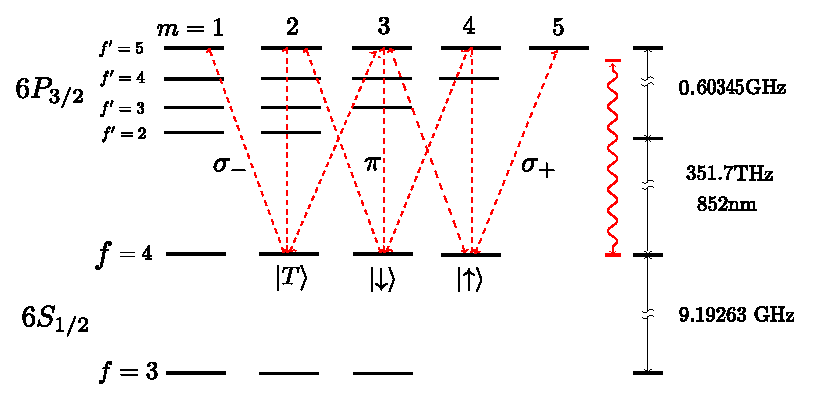
\includegraphics[width=0.75\textwidth]{../media/Figs/D2line_stretchstates}}
\caption[D2 line transitions in the magnetic stretched state space.]{Magnetic stretched state space and some D2 line transitions between $ f=4 $ and $ f'=5 $ manifolds (red dashed lines). }\label{fig:D2line_stretchstates}
\end{figure}

Another useful atomic state of the alkali atoms is the \emph{magnetic stretched state}\index{state!stretched state}, which is defined as a hyperfine state of $ \ket{f,m=f} $ (see Fig.~\ref{fig:D2line_stretchstates}). 
It has the largest magnetic quantum number and be relatively easily prepared with persistent $ \sigma $ pumping transitions, which makes the stretched state a good candidate for precise QND measurements.
In the $ 6S_{1/2} $ ground state levels, we define the fiducial state\index{state!fiducial state} in the $ x $ basis that
\begin{align}
\ket{\uparrow} = \ket{f=4,m_x=4}. 
\end{align}
Following the same trick to find a closed subspace for collective measurement as for the clock states, we define the spin squeezing operator in the $ x $ basis that $ \hat{F}_\perp=\hat{F}_z=\sum_n\hat{f}_z^{(n)} $. 
We want to find a set of states so that applying $ \hat{f}_z $ on the fiducial state will yield the coupled state or $ \ket{\downarrow} $.
That is, $ \hat{f}_z^{(i)}\ket{\uparrow}^{(i)}\rightarrow \ket{\downarrow}^{(i)} $ for each atom.
To satisfy these relations, we define the coupled state\index{state!coupled state}
\begin{align}
\ket{\downarrow} = \ket{f,m_x=f-1}
\end{align}
and 
\begin{align}
\hat{f}_0&=\ket{\uparrow}\bra{\uparrow}+\ket{\downarrow}\bra{\downarrow}\\
\hat{f}_x&=f\ket{\uparrow}\bra{\uparrow}+(f-1)\ket{\downarrow}\bra{\downarrow}\\
\hat{f}_y&=i\sqrt{f/2}(\ket{\downarrow}\bra{\uparrow}-\ket{\uparrow}\bra{\downarrow})\\
\hat{f}_z&=\sqrt{f/2}(\ket{\downarrow}\bra{\uparrow}+\ket{\uparrow}\bra{\downarrow})
\end{align}
in a qubit subspace of the $ f $ hyperfine manifold. These operators only capture a subset of the whole manifold space of the $ f $ hyperfine structure level. Any losses leaked out of the qubit subspace are not tracked. Moreover, they do not provide the information about transfer of coherences~\cite{Norris2014}. Therefore, it is better to extend the subspace to a larger space. 
Assuming initially, all atoms are prepared on the $ \ket{\uparrow} $ state, the spin squeezing operator $ \hat{f}_z $ will transfer some population to the $ \ket{f,m_x=f-1}$ state, but only a tiny fraction on the $ \ket{f,m_x=f-2} $ and sublevels further away from $ \ket{\uparrow} $. We call 
\begin{align}
\ket{T} = \ket{f,m_x=f-2}
\end{align}
as the transfer state\index{state!transfer state}. In the $ \{\ket{\uparrow},\ket{\downarrow},\ket{T} \} $ qutrit subspace, the atomic operators can be truncated from the full space as
\begin{align}
\hat{f}_0&=\ket{\uparrow}\bra{\uparrow}+\ket{\downarrow}\bra{\downarrow}+\ket{T}\bra{T}\\
\hat{f}_x&=f\ket{\uparrow}\bra{\uparrow}+(f-1)\ket{\downarrow}\bra{\downarrow}+(f-2)\ket{T}\bra{T}\\
\hat{f}_y&=i\sqrt{\frac{f}{2}}(\ket{\downarrow}\bra{\uparrow}-\ket{\uparrow}\bra{\downarrow})+i\sqrt{\frac{2f-1}{2}}(\ket{T}\bra{\downarrow}-\ket{\downarrow}\bra{T})\\
\hat{f}_z&=\sqrt{\frac{f}{2}}(\ket{\downarrow}\bra{\uparrow}+\ket{\uparrow}\bra{\downarrow}) + \sqrt{\frac{2f-1}{2}}(\ket{T}\bra{\downarrow}+\ket{\downarrow}\bra{T}).
\end{align}

Processing in the same way as for the clock space, the total atom-light interaction Hamiltonian can be projected onto the stretched qutrit subspace and can be simplified to the form of Eq.~\eqref{eq:heff_chifS}.

Worth noting that, if there is only a transverse linearly polarized electric field at the atom positions, the Hamiltonian may only remain one dominant non-zero term, $ \chi_{33}\hat{F}_z\hat{S}_3 $, which yields a Faraday effect with coupling strength $ \chi_{33} $ due to a vector coupling between the atoms and light.
Especially when the detuning of the probe is large, we can ignore the tensor coupling strength related to $ C_{jj'ff'}^{(2)} $ terms in Eq.\eqref{eq:chippp} as the tensor interaction strength ($ \sim 1/\Delta^2 $) is relatively small compared to the vector interaction strength ($ \sim 1/\Delta $)~\cite{Deutsch2010a}. 
Knowing the form of the Faraday interaction coupling strength $ \chi_{33} $, we can optimize the measurement geometry so that the cooperativity of the Faraday interaction reaches its maximum value. We will discuss more in Chapter~\ref{chap:Faraday}.



\subsection{Spin coherent states, Dicke states and spin squeezed states}
Now, we consider some states of collective spins that will be used for collective quantum measurements. They are spin coherent states, Dicke states and spin squeezed states.

Spin coherent states are the most classical-like quantum state of a collective spin system, which has maximum projection along some axis $ \hat{\mathbf{n}} $. For example, we consider a $ N $-spin-$ \frac{1}{2} $ system in a spin coherent state\index{state!spin coherent state} (SCS) with all spins in $ \ket{\uparrow} $ along the $ x $ axis:
\begin{subequations}\label{eq:SCSJx}
\begin{align}
\ket{J,M_x=J} &=\ket{\uparrow_x}^{\otimes N} = \left(\frac{\ket{\uparrow}+\ket{\downarrow}}{\sqrt{2}}\right)^{\otimes N}\\
&= \sum_{M=-J}^J \left( \begin{matrix}N\\ M \end{matrix} \right) \left( \frac{1}{\sqrt{2}}\right)^{N-M} \left( \frac{1}{\sqrt{2}}\right)^{M} \ket{J,M}
\end{align}
\end{subequations}
which is a binomial distribution of all eigenstates $ \ket{J,M} $. 
Notice that the $ \ket{J,M} $ with $ |M|<J $ are known as the \emph{Dicke states}\index{state!Dicke state}. 
A Dicke state with $ N $ qubits including $ k $ excitations is also defined as~\cite{Dicke1954,Toth2007Detection} 
\begin{align}
\ket{D_k^N} =  \sum_j P_j \left\{\ket{1}^{\otimes k}\ket{0}^{\otimes (N-k)} \right\}\bigg/{\sqrt{\left( \begin{smallmatrix}N\\ k \end{smallmatrix} \right)}},
\end{align}
where $ \sum_j P_j \left\{\cdot\right\} $ denotes the sum over all possible permutations. For example, $ \ket{D_2^3} =\frac{1}{\sqrt{3}}\left(\ket{110}+\ket{101}+\ket{011} \right) $. 

When $ N $ is large, this binomial distribution in Eq.~\eqref{eq:SCSJx} becomes a Gaussian based on the central limit theorem. As a concrete example, we can consider $ N=2 $ case of SCS:
\begin{align}
\ket{\uparrow_x}^{\otimes 2} &= \left(\frac{\ket{\uparrow}+\ket{\downarrow}}{\sqrt{2}}\right)^{\otimes 2}\\
&= \frac{1}{2}\ket{\uparrow\uparrow} +\frac{1}{\sqrt{2}}\left(\frac{\ket{\uparrow\downarrow}+\ket{\downarrow\uparrow}}{\sqrt{2}} \right) + \frac{1}{2}\ket{\downarrow\downarrow}\\
&= \frac{1}{2}\ket{1,1}+\frac{1}{\sqrt{2}}\ket{1,0}+\frac{1}{2}\ket{1,-1}.
\end{align}
Therefore, if we apply a $ J_z $ measurement, we will have a possibility distribution of obtaining $ \pm 1 $ and $ 0 $ with $ P(\pm 1)=\frac{1}{4} $ and $ P(0)=\frac{1}{2} $. As $ N $ increases, the possibility distribution eventually becomes a Gaussian shape, the width of which characterizes the uncertainty of the $ J_z $ measurement. 

%\textcolor{red}{Better to have a measurement distribution plot here.}

In general, a SCS can be treated as a rotated state from the stretched state $ \ket{J,-J} $ 
%(\textcolor{red}{need a plot of the Bloch sphere here}):
\begin{align}
\ket{\theta,\phi} \equiv \hat{D}_{\theta,\phi} \ket{J,-J},
\end{align} 
where the rotation operator with rotation angle $ (\theta,\phi) $ is defined as
\begin{align}
\hat{D}_{\theta,\phi} =e^{-i\theta\hat{n}\cdot \mathbf{J}}=e^{-i\theta (\hat{J}_x\sin \phi - \hat{J}_y\cos \phi) }. 
\end{align}
Note that, for the stretched state along $ \hat{n}_{\theta,\phi} $, $ \hat{n}_{\theta,\phi}\cdot \mathbf{J}\ket{\theta,\phi}=-J\ket{\theta,\phi} $. 
In terms of the standard basis, $ \left\{ \ket{J,M} \right\} $,
\begin{align}
\ket{\theta,\phi} =\sum_{M=-J}^J \frac{\tau^{M+J}}{(1+|\tau|^2)^J} \left( \begin{matrix} 2J\\ M+J\end{matrix}\right)^{1/2} \ket{J,M},
\end{align} 
where $ \tau = \tan \frac{\theta}{2}e^{-i\phi} $. 
When $ \theta=\frac{\pi}{2} $, $ \tau=\frac{1}{\sqrt{2}}e^{-i\phi} $, $ J_z =0$ and the probability distribution of magnetic sublevels obeys the binomial distribution of a fair coin as shown in the example earlier. 
\begin{align}
P_M &= |\bravket{J,M}{\theta=\frac{\pi}{2}}|^2\\
&=\left( \begin{matrix} 2J\\ M+J\end{matrix}\right) \left(\frac{1}{2} \right)^{2J}\left(\frac{1}{2} \right)^{M+J} \Rightarrow \frac{1}{\sqrt{\pi J}} e^{-\frac{M^2}{J}} \quad \text{for} J\rightarrow\infty.
\end{align}
The central limit theorem was applied in the last step to retrieve the Gaussian distribution function with mean zero and variance $ J/2 $. As can be seen, the SCS gives the minimum uncertainty for the $ J_\perp $:
\begin{align}
\expect{\Delta J_\perp} &= \frac{J}{2}=\frac{N}{4}.
\end{align} 
This is known as the \emph{shot noise limit}\index{noise!short noise limit}. 

%Since one can present the density operator of the collective spin state onto the spin coherent basis, 
%\begin{align}
%\hat{\rho} &= \int P(\theta,\phi) \ketbra{\theta,\phi} \mathrm{d}\Omega ,
%\end{align}
%where $ \mathrm{d}\Omega=\sin\theta \mathrm{d}\theta \mathrm{d}\phi $ is the solid angle differential element, and $ P(\theta,\phi) $ is the probability distribution function. In our case, we only consider SCS and spin squeezed states, both of which are Gaussian. The typical representations like P-representation, Q-representation and Wigner-representation of those states are always positive and Gaussian. One can pick anyone of the representations to visualize the probability distribution as a function of $ (\theta,\phi) $ on a generalized Block sphere for the $ 2J+1 $ dimensional collective spin state space. In contrast to the usual Bloch sphere mapping the spin-$ \frac{1}{2} $ or qubit states, the position of the collective spin state on the the generalized Bloch sphere only indicates the mean spin direction and its fluctuation.  
In the SCS case, the isotropic angular uncertainty on the generalized Bloch sphere\index{Bloch sphere} 
%$ \Delta \phi=\Delta \theta $, and 
can be defined by the ratio of the uncertainty of the perpendicular spin direction $ \Delta J_\perp $ to the mean spin length $ J $:
\begin{align}\label{eq:deltaphiJ}
\Delta \phi = \frac{\Delta J_\perp }{\expect{\hat{J}}} = \frac{1}{\sqrt{2J}}=\frac{1}{\sqrt{N}}.
\end{align} 
This limit arises as the classical statistical limit in a system consisting of $ N $ independent particles, and is known as the \emph{standard quantum limit}\index{noise!standard quantum limit}. 
For the SCS, the uncertainties of any two orthogonal angular momentum components that is perpendicular to the spin direction are equal and reaches the minimum value of $ \sqrt{J/2} $ (we set $ \hbar=1 $). 

 
The collective spin state becomes a spin squeezed state (SSS) when the uncertainties of two orthogonal angular momentum components differ from each other and satisfy
\begin{align}
\Delta J_{\perp_1} \Delta J_{\perp_2} &= \frac{J}{2}\\
\Delta J_{\perp_1} = \Delta J_{\perp,min} &< \sqrt{J/2},
\end{align}
where $ \Delta J_{\perp_1} = \Delta J_{\perp,min} $ and $ \Delta J_{\perp_2} = \Delta J_{\perp,max} $ are the two principle axis of the uncertainty shadow on the generalized Bloch sphere\index{Bloch sphere}. 
%On the generalized Bloch sphere, a SCS can be visualized as a blur of circle area on the surface of the sphere. 
%In contrast, a Dicke state is a perfect circle surrounding the sphere with a single project eigenvalue on one axis of the Bloch sphere, which indicates the uncertainty on one direction is zero. 
%A spin squeezed state is a squeezed round or similar to an elliptical blur area on the sphere. It looks like an interim state between a coherent state and a Dicke state.
We plot a SCS\index{state!spin coherent state}, a SSS\index{state!spin squeezed state} and a Dicke state\index{state!Dicke state} on the Bloch sphere\index{Bloch sphere} in Fig.~\ref{fig:collectivestatesonblochsphere}.

A SSS can be created by the nonlinear effect of measurement backaction. We can model this by a weak measurement of one spin component, defined by the Kraus operators~\cite{Deutsch2010a}
\begin{align}\label{KrausOpSq}
\hat{A}_m &= \frac{1}{(2\pi \sigma^2)^{1/4}} e^{-\frac{(m-\hat{J}_z)^2}{4\sigma^2}}
\end{align}
where $ \sigma  $ is the variance of the measurement and defines the resolution of measurement. Given an input state $ \ket{\Psi}_{in} $, the post measurement state becomes
\begin{align}
\left. \ket{\Psi}_{out} \right|_m &= \frac{\hat{A}_m\ket{\Psi}_{in}}{||\hat{A}_m\ket{\Psi}_{in}|| }. 
\end{align}
Ignoring normalization for the moment, expanding $ \ket{\Psi}_{in} = \sum_M C_{M} \ket{J,M} $ in the standard basis
\begin{align}
\ket{\Psi}_{out} &\propto \sum_M e^{-\frac{(m-M)^2}{4\sigma^2}} C_{M} \ket{J,M}.
\end{align}
Therefore, the probability of the output state being conditioned on the measurement $ m $ is 
\begin{align}
P_{M|m} &\propto  e^{-\frac{(m-M)^2}{2\sigma^2}} |C_{M}|^2 = e^{-\frac{(m-M)^2}{2\sigma^2}} P_{M|in}.
\end{align}
If the input state is a SCS with $ J\gg 1 $, the initial $ P_{M|in} $ is well approximated as Gaussian, $ P_{M|in}=e^{-\frac{M^2}{2\Delta J_{in}^2}} $ with $ \Delta J_{in}^2=J/2 $. Thus,
\begin{align}
P_{M|m} \propto e^{-\frac{(M-\bar{M}(m))^2}{2\Delta J_{out}^2}},
\end{align}
where $ \Delta J_{out}^2 =\frac{\Delta J_{in}^2}{1+\xi} $, $ \bar{M}(m)=\frac{m}{1+\xi} $, and $ \xi\equiv \frac{\Delta J_{in}^2}{\sigma^2}=\frac{J}{2\sigma^2} $ which characterizes the measurement backaction and the squeezing effect. The ability to resolve the initial quantum variance of $ J_z $ within the resolution of the meter is the key to QND measurement. 

For a general spin $ F $ system, a squeezed spin state\index{squeezed spin state} may satisfy $ \Delta F_1\Delta F_2=\frac{1}{2} $ and $ \Delta F_1<\Delta F_2 $, where $ \hat{F}_1 $ and $ \hat{F}_2 $ are two collective spin operators. 
Similar to Eq.~\eqref{eq:deltaphiJ}, the isotropic angular uncertainty of the spin-$ F $ system is $ \Delta \phi=  {\Delta F_\perp }/{\expect{\hat{F}_\parallel}}$,
where $ \hat{F}_\parallel $ and $ \hat{F}_\perp $ are the collective atomic angular momentum operators parallel with and perpendicular to the total atomic angular momentum vector on the generalized Bloch sphere\index{Bloch sphere}, respectively.
We call the operator that yields the smaller quadrature as the atomic angular momentum operator $ \hat{F}_\perp $ and 
recall the spin squeezing parameter defined by Wineland {\emph{et al.}}~\cite{Wineland1992,Baragiola2014},
\begin{align}\label{eq:zeta2_general}
\zeta^2 &\equiv \frac{\Delta \phi^2}{\Delta \phi^2_{SCS}}=\frac{\expect{\hat{F}_\parallel(t=0)}^2}{\expect{\Delta F_\perp^2(t=0)}} \frac{\expect{\Delta F_\perp^2}}{\expect{\hat{F}_\parallel}^2}
\end{align}
requires to calculate the expectation value $ \expect{\hat{F}_\parallel} $ and the variance $ \Delta F_\perp^2 $. 
Assume the atom number is $ N_A $, these two collective quantities can be decomposed into microscopic quantities by 
\begin{align}
\expect{\Delta F_\perp^2} &= N_A \expect{\Delta f_\perp^2}+\frac{N_A(N_A-1)}{2}\left. \expect{\Delta f_\perp^{(i)}\Delta f_\perp^{(j)}}_s\right|_{i\neq j}\label{eq:DeltaFz2_general}\\
\expect{\hat{F}_\parallel } &= \sum_i^{N_A} \expect{\hat{f}_\parallel ^{(i)}}=N_A \expect{\hat{f}_\parallel},\label{eq:expectFx_general}
\end{align}
where the first term of Eq.~\eqref{eq:DeltaFz2_general} and Eq.~\eqref{eq:expectFx_general} are solely determined by a symmetric sum over $N_A$ identical spin-$f$ single-body operators, $ \hat{f}_\perp=\hat{f}_\perp^{(i)} $ and $ \hat{f}_\parallel=\hat{f}_\parallel^{(i)} $ with atom labels $ i=1,\cdots,N_A $; the second term of Eq.~\eqref{eq:DeltaFz2_general} is determined by symmetric two-body covariance terms, $ \left.\expect{\Delta f_\perp^{(i)}\Delta f_\perp^{(j)}}_s\right|_{i\neq j}=\expect{\Delta f_\perp^{(1)}\Delta f_\perp^{(2)}}_s\equiv \expect{\hat{f}_\perp^{(1)}\hat{f}_\perp^{(2)}}_s-\left( \expect{\hat{f}_\perp^{(1)}} \expect{\hat{f}_\perp^{(1)}}\right)_s $, which correspond to the pairwise entanglement among atoms and eventually yield spin squeezing~\cite{Wang2003Spin}.
Above, we have assumed there is a pairwise exchange symmetry among atoms so that we only care about the symmetrized quantities like $ \expect{\Delta f_\perp^{(1)}\Delta f_\perp^{(2)}}_s=\left(\expect{\Delta f_\perp^{(1)}\Delta f_\perp^{(2)}} + \expect{\Delta f_\perp^{(2)}\Delta f_\perp^{(1)}} \right)/2 $. 


% Rewrite the Hamiltonian in the Stokes and collective spin representation. 
\section{Spin squeezing induced by QND measurement}
To explain how a quantum measurement can generate a spin squeezed state, we consider the polarization spectroscopy measurement setup that the measurement of the light's polarization state is used to infer the state of atoms (spins). We take the example of a birefringence-rotation--based QND measurement and spin squeezing protocol to map the collective operators to the quatratures of a phase space plane under the \emph{Holstein-Primakoff approximation}\index{Holstein-Primakoff approximation}. 
A similar analog has been done for a Faraday-rotation--based spin squeezing protocol in Refs.~\cite{Norris2014,Baragiola2014Open}. 

The measurement setting is the following. 
$ N_A $ atoms are trapped on the $ x $ axis of a waveguide on a two-side chain of optical lattices. All atoms are prepared to be the $ \ket{\uparrow_x}=(\ket{\uparrow}+\ket{\downarrow})/\sqrt{2} $ state in the clock space. The probe light is initially polarized along the diagonal direction of the $ xy $ plane and is adiabatically connected to the $ D $ mode of the waveguide. As we will discuss in Chapter~\ref{chap:birefringence}, the guided modes will experience a birefringence rotation on the \Poincare sphere under some magic frequency~\cite{Qi2016}. 
We consider an $ S_3 $ measurement of the output light to determine the $ J_z $ project of the collective spin state. 
The interaction Hamiltonian can been derived in Eq.~\eqref{eq:Heffupdown}.

%We define the pseudo-spin operator in the corresponding clock space for one atom as $ \mathbf{j}=\frac{\boldsymbol{\sigma}}{2} $. We will use  the following spin components, which can be expressed as
%\begin{align}
%\hat{j}_z &= \frac{1}{2} \Big( \op{\uparrow}{\uparrow} - \op{\downarrow}{\downarrow}  \Big), \\
%\hat{j}_0 &= \frac{1}{2} \Big( \op{\uparrow}{\uparrow} + \op{\downarrow}{\downarrow}  \Big).
%\end{align}
%The quantization axis is chosen to be the $ x $ axis. For a collective spin system with $ N_A $ atoms, the pseudo-spin angular momentum operator can be defined as
%\begin{align}
%\mathbf{J} &=\sum_i^{N_A}\mathbf{j}^{(i)}=\frac{1}{2}\sum_i^{N_A} \boldsymbol{\sigma}^{(i)}\\
%\mathbf{J}_+ &=\sum_i^{N_A} \boldsymbol{\sigma}^{(i)}_+.
%\end{align}
%The maximum possible angular momentum is $ J=\frac{N_A}{2} $. Each $ J_z $ measurement will yield an eigenvalue ranging from $ -\frac{N_A}{2} $ to $ \frac{N_A}{2} $.  This subspace is unique with dimension $ D=2J+1=N_A+1 $, and is symmetric with respect to exchange of any two individual spins. The different total $ J $'s of the collective spin-$ \frac{1}{2} $ system support "irreducible" matrix representation of the $ SU(2) $ group. The spin operator components satisfy the commutator relationship that $ [J_i,J_j]=i\varepsilon_{ijk}J_k $. Therefore, any pair of the spin operators obey the Heisenberg uncertainty relationship which--for $ \Delta J_x^2 $ and $ \Delta J_y^2 $--is given by 
%\begin{align}
%\Delta J_x^2\Delta J_y^2 &\ge \frac{1}{4}\langle J_z^2\rangle \\
%\expect{\Delta J_x} &=\expect{\Delta J_y}=\expect{\Delta J_{\perp}}=\sqrt{\frac{J(J+1)-M^2}{2}}.
%\end{align}
%The minimum uncertainty for $ \ket{J,M=\pm J} $ gives $ \Delta J_\perp=\Delta J_x=\Delta J_y = \sqrt{\frac{J}{2}} $ while $ \expect{J_\parallel}=\expect{J_z^2}=M^2=J^2 $. 

This birefringence measurement protocol uses an input laser with the polarization state $ \vec{D}=\left( \vec{H}+\vec{V}\right)/\sqrt{2} $, which is pointing along the $ S_2 $ direction on the \Poincare sphere. For a large number of photon flux incidence, we can set 
\begin{subequations}\label{eqs:cohaHV}
\begin{align}
\hat{a}_H &\rightarrow i\sqrt{\frac{\dot{N}_L}{2}} + \hat{a}_H\\
\hat{a}_V &\rightarrow i\sqrt{\frac{\dot{N}_L}{2}} + \hat{a}_V,
\end{align}
\end{subequations}
where each operator has a classical part associated with the photon flux number, $ \dot{N}_L $, and a quantum operator part to include the quantum fluctuations of photons, which lead to the \emph{shot noise}\index{noise!shot noise}. In the case of $ \dot{N}_L\gg \sqrt{\dot{N}_L}\gg 1 $, the Stokes operators can be given by
\begin{align}
\hat{S}_1 &= \frac{1}{2}\!\left[ \!\Big(\!\! -\! i\sqrt{\frac{\dot{N}_L}{2}} \!+\! \hat{a}_H\dg \!\Big)\! \Big(\! i\sqrt{\frac{\dot{N}_L}{2}} \!+\! \hat{a}_H \!\Big) \!-\!  \Big(\!\! -\! i\sqrt{\frac{\dot{N}_L}{2}} \!+\! \hat{a}_V\dg\!\Big) \! \Big(\! i\sqrt{\frac{\dot{N}_L}{2}} \!+\! \hat{a}_V \!\Big)\! \right]\\
&= \sqrt{\frac{\dot{N}_L}{2}} \frac{i}{\sqrt{2}} \left[\frac{\hat{a}_H\dg-\hat{a}_V\dg}{\sqrt{2}} - \frac{\hat{a}_H-\hat{a}_V}{\sqrt{2}} \right] + \frac{1}{2} \Big( \hat{a}_H\dg \hat{a}_H -  \hat{a}_V\dg \hat{a}_V \Big)\\
&\approx \sqrt{\frac{\dot{N}_L}{2}} \frac{i}{\sqrt{2}} \left( \hat{a}_{\bar{D}}\dg-\hat{a}_{\bar{D}}\right)\\
&= \sqrt{\frac{\dot{N}_L}{2}} \hat{P}_{\bar{D}},\\
\hat{S}_3 &= \frac{1}{2i}\! \left[\! \Big(\!\! -\! i\sqrt{\frac{\dot{N}_L}{2}} \!+\! \hat{a}_H\dg \!\Big)\! \Big(\! i\sqrt{\frac{\dot{N}_L}{2}} \!+\! \hat{a}_V\! \Big) \!-\!  \Big( \!\!-\! i\sqrt{\frac{\dot{N}_L}{2}} \!+\! \hat{a}_V\dg \!\Big)\! \Big(\! i\sqrt{\frac{\dot{N}_L}{2}} \!+\! \hat{a}_H \!\Big)\! \right]\\
&= \sqrt{\frac{\dot{N}_L}{2}}  \frac{1}{\sqrt{2}}\left[ \frac{\hat{a}_H\dg-\hat{a}_V\dg}{\sqrt{2}} + \frac{\hat{a}_H-\hat{a}_V}{\sqrt{2}} \right] +\frac{1}{2i} \Big( \hat{a}_H\dg \hat{a}_V -  \hat{a}_V\dg \hat{a}_H \Big)\\
&\approx \sqrt{\frac{\dot{N}_L}{2}} \hat{X}_{\bar{D}},\label{eq:S3_XD}\\
\hat{S}_2 &\approx \frac{\dot{N}_L}{2},\\
\hat{S}_0 &\approx \frac{\dot{N}_L}{2},
\end{align}
where we have defined $ \hat{a}_{\bar{D}} = \frac{\hat{a}_H -\hat{a}_V}{\sqrt{2}} $ as the photon annihilation operator of the anti-diagonal linearly polarized light modes, and $ \hat{P}_{\bar{D}}=\frac{\hat{a}_{\bar{D}}-\hat{a}_{\bar{D}\dg}}{i\sqrt{2}} $ and $ \hat{X}_{\bar{D}}=\frac{\hat{a}_{\bar{D}}+\hat{a}_{\bar{D}\dg}}{\sqrt{2}} $ as the two quadratures in the phase space of the complex amplitude represented by $ \hat{a}_{\bar{D}} $. The approximation we made above is known as \emph{Holstein-Primakoff approximation}\index{Holstein-Primakoff approximation}. Using this approximation, the uncertainty area on the \Poincare sphere can be mapped to a flat phase plane. 


Notice that, the $ \hat{S}_1 $ and $ \hat{S}_3 $ still satisfy the usual $ SU(2) $ Lie algebra relationship that 
\begin{align}
[\hat{S}_3,\hat{S}_1] = i \hat{S}_2 \approx i\frac{\dot{N}_L}{2}
\end{align}
which is important for us to choose $ \hat{S}_1 $ as the rotation axis and $ \hat{S}_3 $ as the observation axis on the \Poincare sphere for our QND measurement as will be discussed later. 



Similarly, when the atom number is large, one can also map the angular momentum/spin operators to the quadrature operators. However, we will try to avoid applying this approximation to the spin operators, since the total number of the atoms are not too large in the context of this piece of dissertation work. 



Now, we recall the spin operators $ \mathbf{j}={\boldsymbol{\sigma}}/{2} $ with components
\begin{align}
\hat{j}_z &= \frac{1}{2} \Big( \op{\uparrow}{\uparrow} - \op{\downarrow}{\downarrow}  \Big), \\
\hat{j}_0 &= \frac{1}{2} \Big( \op{\uparrow}{\uparrow} + \op{\downarrow}{\downarrow}  \Big).
\end{align}
We rewrite the effective Hamiltonian of the spin-photon system described in Eq.~\eqref{eq:Heffupdown} in terms of the Stokes and spin operators for individual atoms, 
\begin{align}
\op{\uparrow}{\uparrow} &= \hat{j}_z + \hat{j}_0, \\ \op{\downarrow}{\downarrow} &= \hat{j}_0 - \hat{j}_z,\\
\hat{a}_H\dg \hat{a}_H &= \hat{S}_0 + \hat{S}_1,\\
\hat{a}_V\dg \hat{a}_V &= \hat{S}_0 - \hat{S}_1.
\end{align}
We obtain
\begin{align}
H_{\rm eff} = \hbar \Big\{ & \big( \chi_{H,\uparrow} + \chi_{H,\downarrow} + \chi_{V,\uparrow} + \chi_{V,\downarrow}\big) \hat{J}_0 \hat{S}_0 \nonumber \\
+ & \big( \chi_{H, \uparrow} + \chi_{H,\downarrow} - \chi_{V,\uparrow} - \chi_{V,\downarrow} \big)  \hat{J}_0 \hat{S}_1 \nonumber \\
+ & \big( \chi_{H,\uparrow} - \chi_{H,\downarrow} + \chi_{V,\uparrow} - \chi_{V,\downarrow} \big)  \hat{J}_z \hat{S}_0 \nonumber \\
+ & \big( \chi_{H,\uparrow} - \chi_{H,\downarrow} - \chi_{V,\uparrow} + \chi_{V,\downarrow} \big)  \hat{J}_z \hat{S}_1\Big\}\\
=\hbar \Big\{ & \left[ \big( \chi_{H,\uparrow} + \chi_{H,\downarrow}\big) + \big(\chi_{V,\uparrow} + \chi_{V,\downarrow}\big) \right] \hat{J}_0 \hat{S}_0 \nonumber \\
+ & \left[ \big( \chi_{H, \uparrow} + \chi_{H,\downarrow}\big) - \big( \chi_{V,\uparrow} + \chi_{V,\downarrow} \big)\right]  \hat{J}_0 \hat{S}_1 \nonumber \\
+ & \left[ \big( \chi_{H,\uparrow} - \chi_{H,\downarrow}\big) + \big(\chi_{V,\uparrow} - \chi_{V,\downarrow} \big) \right] \hat{J}_z \hat{S}_0 \nonumber \\
+ & \left[ \big( \chi_{H,\uparrow} - \chi_{H,\downarrow}\big) - \big(\chi_{V,\uparrow} - \chi_{V,\downarrow} \big) \right]  \hat{J}_z \hat{S}_1\Big\}
\end{align}
The first term is an overall scalar shift and thus does not contribute to the relative dynamics.  The second term is a constant birefringence and can be cancelled with a compensating waveplate as long as the atom number remains constant. 
%which is usually the case when the trapping time is fairly large compared to the measurement time. Typically, if we choose to have the atoms on the bisection line of the $ x $- and $ y $-axes, we would have the coupling strengthen canceled. It will also remove the forth term in the equation above. The first two terms can be also be canceled when we have the detuning approximately equally biased for the $ f=3 $ and $ f=4 $ ground states. 
%For example, we  can choose $ \Delta_3=-4.6 $ GHz and $ \Delta_4=4.6 $ GHz to the $ 6P_{1/2} $ excited state sublevels to satisfy this condition, where the hyperfine splitting of the excited state can be ignored ($ ~500 $ MHz) compared to the detuning. However, we would like to leave the choice of detuning to control the third and fourth terms as will be discussed consequently. 

The final term describes the QND Faraday interaction we wish to isolate (similar to the Faraday interaction since we choose to use the $ x $ axis as the quantization axis), but this requires dealing with the third term that describes the effect of the scalar light shift on the rotation of the pseudo-spin, which injects photon fluctuation noise to the measurement signal.  Cancelling the third term amounts to enforcing the condition that
\begin{align}\label{eq:magiccondition}
	\chi_{H,\uparrow} - \chi_{H,\downarrow} = \chi_{V,\downarrow} - \chi_{V,\uparrow} ,
\end{align}
which can be satisfied if we carefully choose the detuning of the probe light. The wavelength chosen to cancel the third term is atom position related, since the condition is determined by the effective mode areas which may have different ratios for the $ H $ and $ V $ modes at different locals. We call the exact wavelength to satisfy this condition as the \emph{magic wavelength}\index{magic wavelength}, which will be discussed in details in the next chapter. Using a magic frequency, we can achieve an interaction Hamiltonian of the following form,
\begin{align}
	H_{\rm LS} = \hbar \chi_{\rm eff} \hat{J}_z \hat{S}_1
\end{align}
where $\chi_{\rm eff} = 2(\chi_{H,\uparrow} - \chi_{H,\downarrow})$.  

Using this, we find the spin state as an eigenvalue projected onto the $ J_z $ axis by measuring the rotation angle of the probe around the $ S_1 $ axis after the photon-atom interaction. To implement this measurement, we use the $ \hat{S}_3 $ Stokes measurement. As a result of the backaction of the polarization measurement, there generates a squeezing effect to the collective spin state which reduces the uncertainty of measurement output of $ \expect{\hat{J}_z} $. To see this, we assume the photon number is large and apply the Holstein-Primakoff approximation\index{Holstein-Primakoff approximation} to set $ \hat{S}_1=\sqrt{\frac{\dot{N}_L}{2}}\hat{P}_{\bar{D}} $ and $ \hat{S}_3=\sqrt{\frac{\dot{N}_L}{2}}\hat{X}_{\bar{D}} $. Now the effective Hamiltonian can be written as
\begin{align}\label{eq:HeffJzPD}
H_{\rm eff} = \hbar \chi_{\rm eff} \sqrt{\frac{\dot{N}_L}{2}}\hat{J}_z \hat{P}_{\bar{D}}. 
\end{align}
The $ \hat{S}_3 $ measurement is achieved through sending the signal light to one input port of a beam splitter along as a vacuum input on the other input port and then performing a balanced Homodyne measurement of the $ X_{\bar{D}} $ quadrature. The equivalent Kraus operator conditional on this measurement is 
\begin{align}
\hat{A}_{X_{\bar{D}}} &= \bra{X_{\bar{D}}} e^{-i\chi_{\rm eff} \sqrt{\frac{\dot{N}_L}{2}}\hat{J}_z \hat{P}_{\bar{D}}T} \ket{0}\propto \exp\left\{ -\frac{\kappa T}{4}(m-\hat{J}_z)^2 \right\},
\end{align} 
where $ m=\frac{X_{\bar{D}}}{\chi_{\rm eff} \sqrt{\dot{N}_LT/2}} $ is the measurement outcome in angular momentum units, and $ \kappa =\chi_{\rm eff}^2\dot{N}_L $ is the integrated measurement strength per spin in a measurement period $ T $. The shot noise resolution of the QND measurement is $ \sigma^2=\frac{1}{\kappa T} $. The Kraus operator is exactly the same as Eq.~\eqref{KrausOpSq} to generate a spin squeezing
 state. For a SCS input state, the output state probability distribution is given by 
 %(from Ben's dissertation)
%\begin{align}
%P(\hat{X}_L=x) = \exp\left[\frac{-(x\tau)^2}{2(\frac{\tau}{2}+\chi_{\rm eff}\Delta J_z^2)} \right].
%\end{align}
%The measurement probabilities have been expressed in terms of $ x\tau $, since the measurements involve integrating the output quadrature over the duration $ \tau $. The variance of measurement outcomes increases through the addition of atomic projection noise. 
\begin{align}
P_{M|m} \propto e^{-\frac{(M-\bar{M}(m))^2}{2\Delta J_{out}^2}},
\end{align}
where the uncertainty of measurement $ \Delta J_{out}^2 =\frac{\Delta J_{in}^2}{1+\xi}=\frac{J}{2(1+\xi)} $ is reduced when $ \xi\equiv \frac{\Delta J_{in}^2}{\sigma^2}=\frac{J}{2\sigma^2}=\frac{\chi_{e\!f\!f}^2}{4}N_A\dot{N}_LT \gg 1$. 
The parameter $ \xi $ is proportional to $ \kappa T $ and indicates how much the state is squeezed after the measurement in time $ T $. 
Therefore, without considering the decoherence effect, a larger coupling strength $ \chi_{\rm eff} $ or measurement strength $ \kappa $ will yield a stronger squeezing effect.


%\subsection{Quantum dynamics of continuous measurement and spin squeezing under the Holstein-Primakoff approximation}
%
%Following the example above, the measurement operator, Eq.~\eqref{eq:S3_XD}, after the probe light interacting with the ensemble of atoms can be given by
%\begin{align}
%\hat{\mathcal{M}} &= \sum_n^{N_A}\sqrt{\frac{\dot{N}_L}{2}} \int_0^T \mathrm{d}t' \hat{X}_{\bar{D}}^{\rm out} (z_D,t'-(z_{D}-z_n')/v_p),\label{eq:Mxout}
%\end{align}
%where $ T $ and $ Z_D $ are the integration time and position of the detector, $ z_n' $ is the $ z $-coordinate of the $ n $-th atom. 
% 
%
%For each atom, using the effective Hamiltonian that causes the birefringence effect, 
%Eq.~\eqref{eq:HeffJzPD}, one can find the equation of motion for the quadrature operator $ \hat{X}_{\bar{D}} $ to be
%\begin{align}
%\dt{\hat{X}_{\bar{D}}(z,t)} &= -\frac{i}{\hbar} \left[ \hat{H}_{\rm eff},\hat{X}_{\bar{D}} \right] \\
%\Leftrightarrow \pp{\hat{X}_{\bar{D}}(z,t)}{t}+v_g\pp{\hat{X}_{\bar{D}}(z,t)}{z} &=  \chi_{\rm eff} \sqrt{\frac{\dot{N}_L}{2}} \hat{J}_z.
%\end{align}
%A formal solution can be given by
%\begin{align}
%\hat{X}_{\bar{D}} (z,t) &= \hat{X}_{\bar{D}}(0,t-z/v_p) + \sqrt{\frac{\kappa}{2}}\hat{J}_z(t-(z-z'_n)/v_p)\Theta(z-z'_i),
%\end{align} 
%where the measurement strength per atom is defined as $ \kappa = \chi_{\rm eff}^2 \dot{N}_L $. 
%
%Using the result above, Equ.~\ref{eq:Mxout} gives
%\begin{align}
%\frac{\hat{\mathcal{M}}(T)}{N_A} &= \sqrt{\frac{\dot{N}_L}{2}}\int_0^T\mathrm{d}t \hat{X}_{\bar{D}}(0,t-z_D/v_p) +  \sqrt{\frac{\kappa\dot{N}_L}{4}}\int_0^T\mathrm{d}t\hat{J}_z(t)\\
%&\approx \sqrt{\frac{\dot{N}_L}{2}}\int_0^T\mathrm{d}t \hat{X}_{\bar{D}}(0,t-z_D/v_p) + T\sqrt{\frac{\kappa\dot{N}_L}{4}}\hat{J}_z(0).
%\end{align}
%In the last step, we have used the fact that all atoms around a waveguide are interacting with the probe light in the same manner, and we have assumed the transition time of the light passing through the ensemble of atoms is much shorter than the atomic dynamics and the sampling time of the detector. 
%
%Since the setup of the photon detectors implies a vacuum state of the photonic operators, we may set $ \expect{\int_0^Tdt\hat{X}_{\bar{D}}(0,t-z_D/v_p)}=0 $. The mean value of the measurement can be given by 
%\begin{align}
%\expect{\hat{\mathcal{M}}}(T) &\approx N_AT\sqrt{\frac{\kappa\dot{N}_L}{4}}\expect{\hat{J}_z(0)}.
%\end{align}
%
%The variance of the measurement can be described by
%\begin{align}
%\Delta \mathcal{M}^2(T) &= \expect{\hat{\mathcal{M}}^2}-\expect{\hat{\mathcal{M}}}^2\\
%&= N_A^2 \frac{\dot{N}_L}{2}\int_0^T\mathrm{d}t \int_0^T\mathrm{d}t'  \expect{\Delta\hat{X}_{\bar{D}}(0,t-z_D/v_p)\Delta\hat{X}_{\bar{D}}(0,t'-z_D/v_p)} \nonumber\\
%&\quad + N_A^2 \frac{\kappa\dot{N}_L}{4} \int_0^T\mathrm{d}t \int_0^T\mathrm{d}t'\expect{\Delta\hat{J}_z(t)\Delta\hat{J}_z(t')}\\
%&\approx \frac{N_A^2\dot{N}_LT}{4} + \frac{\kappa N_A^2\dot{N}_LT^2}{4} \Delta\hat{J}_z^2(0)\\
%&\equiv \Delta \mathcal{M}_{\rm SN}^2 + \Delta\mathcal{M}_{\rm PN}^2.
%\end{align}
%To derive the result above, we have used the fact that the covariance $ \expect{\Delta\hat{X}_{\bar{D}}(0,t-z_D/v_p)\Delta\hat{X}_{\bar{D}}(0,t'-z_D/v_p)}\equiv \expect{\hat{X}_{\bar{D}}(0,t-z_D/v_p)\hat{X}_{\bar{D}}(0,t'-z_D/v_p)}-\expect{\hat{X}_{\bar{D}}(0,t-z_D/v_p)}\expect{\hat{X}_{\bar{D}}(0,t'-z_D/v_p)}=\delta(t-t')/2 $ for the vacuum fluctuations, which leads to the vacuum shot noise $ \Delta \mathcal{M}_{\rm SN}^2=\frac{N_A^2\dot{N}_LT}{4} $. The additional projection noise, $ \Delta\mathcal{M}_{\rm PN}^2=\frac{\kappa N_A^2\dot{N}_LT^2}{4} \Delta\hat{J}_z^2(0) $, is the signal coming from the variance of the $ z $-projection of the collective spin state.  
%
%The parameter $ \xi $ can be defined as the ratio between the projection noise and the shot noise. Therefore, we have
%\begin{align}
%\xi = \frac{\Delta\mathcal{M}_{\rm PN}^2 }{ \Delta \mathcal{M}_{\rm SN}^2}= \kappa T \Delta J_z^2(0).
%\end{align}
%This parameter characterizes the squeezing due to the measurement backaction. It implies that, with a strong atom-light coupling ($ \kappa $), the squeezing effect can be enhanced. 
%
%\section{Spin squeezing dynamics under a continuous measurement}
%To study the spin dynamics under a continuous measurement, we formally define a stochastic master equation of the atomic ensemble by~\cite{Gardiner2004}
%\begin{align}\label{eq:totaldrhodt}
%\mathrm{d}\hat{\rho}=\left.\mathrm{d}\hat{\rho}\right|_{op} + \left.\mathrm{d}\hat{\rho}\right|_{QND}.
%\end{align}
%It includes two collective spin dynamic processes. 
%The first process is the optical pumping dynamics on each individual atom $n$ positioned at $\br'$ which yields the $\mathrm{d}\hat{\rho}|_{op}=\sum_n^{N_A} \left.\mathrm{d}\hat{\rho}^{(n)}\right|_{op} $ term given by
%\begin{align}
%&\quad\left.\mathrm{d}\hat{\rho}^{(n)}\right|_{op} =\gamma_s\mathcal{D}^{(n)}\mathrm{d}t\\
%&= -\frac{i\gamma_s}{\hbar} \left\{\hat{h}_{\rm eff},\hat{\rho}^{n} \right\}\mathrm{d}t + \gamma_s\sum_q \hat{W}_q(\br')\hat{\rho}^{i}\hat{W}_q^\dagger(\br')\mathrm{d}t,
%\end{align}
%where the characteristic photon scattering rate $ \gamma_s\equiv \frac{\Gamma\Omega^2}{4\Delta_{\rm eff}}=\frac{\sigma_0}{A_{in}}\frac{\Gamma^2}{4\Delta_{\rm eff}^2}\dot{N}_L $ with the effective input mode area $ A_{in}=1/n_g|\mathbf{u}_{\mathrm{in}}(\br'\!_\perp)|^2 $ and the effective detuning $ \Delta_{\rm eff} $ is defined according to the type of interactions on the order of $ \Delta_{ff'}=\omega-\omega_{ff'} $, where $ \omega_{ff'} $ is the resonance angular frequency between the ground hyperfine structure level $ f $ and the excited hyperfine structure level $ f' $~\cite{Deutsch2010a,Qi2016,Qi2017Enhanced}.
%$\gamma_s$ characterizes the rate of decoherence dynamics and is proportional to the local photon flux of the probe light, $ \dot{N}_L $. The Rabi frequency can be calculated in the following manner. We take the example of the birefringence-effect--based QND measurement protocol discussed in the last section, and the following results hold for classical light input cases, in general.
%In birefringence protocol case, the input light is classical with a large photon flux, and hence we can turn the photon and electric field operators into C-numbers as being derived:
%\begin{align}
%\hat{a}_{H/V} &\rightarrow i\sqrt{\frac{\dot{N}_L}{2}} \\
%\mathbf{E}^{(+)}_L(\mathbf{r}') &\rightarrow i\mathcal{E}_L^{(+)}(\br')\mathbf{e}_L  
%\end{align}
%with the polarization vector and field amplitude 
%\begin{align}
%\mathbf{e}_L &= [\mathbf{u}_H(\br'\!\!_\perp)+\mathbf{u}_V(\br'\!\!_\perp)]/\sqrt{|\mathbf{u}_H(\br'\!\!_\perp)|^2+|\mathbf{u}_V(\br'\!\!_\perp)|^2} \\
%\mathcal{E}_L^{(+)} (\br') &= \sqrt{\frac{2{\pi}\hbar\omega_0}{v_g}\dot{N}_L \left[ |\mathbf{u}_{\rm in}(\br'\!_\perp)|^2 \right]}.
%\end{align}
%The Rabi frequency can then be calculated by
%\begin{align}
%\Omega (\br') &= \frac{2\bra{J'}| d |\ket{J}\mathcal{E}_L^{(+)}(\br')}{\hbar}.
%\end{align}
%
%
%The second term on the right-hand side of Eq.\eqref{eq:totaldrhodt} gives rise to the collective spin dynamics due to QND measurement,
%\begin{align}
%\left.\mathrm{d}\hat{\rho}\right|_{QND} &= \sqrt{\frac{\kappa}{4}}\mathcal{H}\left[\hat{\rho} \right]\mathrm{d}W + \frac{\kappa}{4}\mathcal{L}\left[ \hat{\rho}\right]\mathrm{d}t.
%\end{align}
%Above, we have defined the measurement strength $\kappa \equiv |\chi|^2\dot{N}_L\equiv \frac{\sigma_0A_{in}}{A_{\rm eff}^2}\gamma_s $ determining the rate of the spin squeezing in absence of decoherent processes, where $\dot{N}_L$ is the photon number flux, $\chi$ is the light-atom coupling strength and $A_{\rm eff}$ is the effective interaction mode area which can be specified for a particular QND measurement protocols. We have also assumed the measurement backation is a stochastic Weiner process where $\mathrm{d}W$ is the increment satisfying $\mathrm{d}W^2 = \mathrm{d}t$. The conditional dynamics responding to the measurement evolve under the superoperator
%\begin{align}
%\mathcal{H}\left[ \hat{\rho}\right] &= \hat{F}_\perp\hat{\rho} + \hat{\rho}\hat{F}_\perp -2\expect{\hat{F}_\perp}\hat{\rho}
%\end{align}
%and the collective Lindblad map due to the direct photon scattering of the guided modes from the atoms
%\begin{align}
%\mathcal{L}\left[ \hat{\rho} \right] &= \hat{F}_\perp\hat{\rho}\hat{F}_\perp-\frac{1}{2}\left(\hat{\rho}\hat{F}_\perp^2+\hat{F}_\perp^2\hat{\rho} \right)=\frac{1}{2}\left[\hat{F}_\perp,\left[\hat{\rho},\hat{F}_\perp \right] \right].
%\end{align}
%
%With the equations of motion defined above, one can then solve the expectation values of collective operators and their covariances. Once we solve the time-dependent quantities of $ \expect{\Delta F_\perp^2} $ and $ \expect{\hat{F}_\parallel} $ based on Eqs.~\eqref{eq:DeltaFz2_general} and~\eqref{eq:expectFx_general}, the dynamics of spin squeezing can then be determined using Eq.~\eqref{eq:zeta2_general}. 
%Solving only the collective operator dynamics may not help us understand the physics process in the single-atom level. 
%In practice, to study the correlations and self-evolutions of atoms due to the measurement backaction, we usually solve the microscopic operator dynamics of $ \hat{f}_i $ and their two-body covariances. Even better to be computational efficient, we can also solve the dynamics of the expectation values of the one-body $ \hat{\sigma}_{ba}=\ket{b}\bra{a} $ operators and the two-body covariances $ \expect{\Delta \sigma_{ba}^{(1)}\Delta\sigma_{dc}^{(2)}}  $. Using the microscopic operator dynamics solution, we can easily find the collective operator and spin squeezing dynamics based on their definitions. 
%
%As shown in the equations above, the spin squeezing dynamics is a competition between the coherent squeezing process and all decoherent processes which are characterized by $\kappa$ and $\gamma_s$, respectively. 
%If we define an effective cooperativity, $ C_1 $, or optical depth (OD) per atom, OD$ _{\rm eff}/N_A $, quantity for the spin squeezing dynamics by
%\begin{align}
%C_1=\frac{\mathrm{OD}_{\rm eff}}{N_A} \equiv \frac{\kappa}{\gamma_s}=\frac{\sigma_0A_{in}}{A_{\rm eff}^2},
%\end{align}
%the peaking spin squeezing dynamics can then be characterized by $C_1=\frac{\mathrm{OD}_{\rm eff}}{N_A}$, and the geometry of the spin squeezing protocol can then be roughly designed with the goal to maximize $C_1$ by minimizing $A_{in}$ and maximizing the effective interaction area $A_{\rm eff}$. 
%We will discuss the definitions and details of these quantities in the next two chapters for concrete examples. 



%Hence the master equation describing the expectation values of an arbitrary Hermitian and one-body operator $ \hat{O}^{(i)} $ evolves as
%\begin{align}
%\!\!\!\!\!\!\!\!\!\! \dt{\expect{\hat{O}^{(i)} }} &= \dt{}\tr\left[\hat{\rho}^{(i)}\hat{O}^{(i)} \right]=\tr\left[\dt{\hat{\rho}^{(i)}}\hat{O}^{(i)} \right]=\tr\left[\mathcal{D}^{(i)}(\hat{\rho}^{(i)})\hat{O}^{(i)} \right]\\
%&= \tr\left[\! -\frac{i}{\hbar}\left(\hat{O}^{(i)}\hat{H}_{\rm loss}^{(i)}\!-\! \hat{H}_{\rm loss}^{(i)\dagger}\hat{O}^{(i)}  \right)\!\hat{\rho}^{(i)} \!+\! \!\sum_{F_a,F_b,q} \!\! \!\hat{W}_q^{F_bF_a\dagger}(\br_i) \hat{O}^{(i)} \hat{W}_q^{F_bF_a}(\br_i)\hat{\rho}^{(i)} \right]\\
%&=-\frac{i}{\hbar}\expect{\left[\hat{O}^{(i)}\hat{H}_{\rm loss}^{(i)} \!-\! \hat{H}_{\rm loss}^{(i)\dagger}\hat{O}^{(i)}\right]}+ \expect{\!\!\sum_{F_b,F_a,q}\!\! \hat{W}_q^{F_bF_a\dagger}(\br_i) \hat{O}^{(i)} \hat{W}_q^{F_bF_a}(\br_i) }\\
%&= \expect{\mathcal{D}^{(i)\dagger}\left[\hat{O}^{(i)} \right] }
%%&= -\gamma_s^+\expect{\hat{O}} \!-\! \frac{\gamma_s^-}{2}\sum_i^{N_A}\expect{\!\left\{ \hat{\sigma}_z^{(i)},\hat{O} \right\}\!} \!+\! \expect{\!\!\sum_{F_b,F_a,i}\!\! \gamma_{F_bF_a} \op{F_b,0}{F_a,0}^{(i)} \hat{O} \op{F_a,0}{F_b,0}^{(i)} },
%\end{align}
%%In fact, to ensure $ \hat{\rho}^{(i)} $ Hermitian, Equ.~\eqref{eq:drhoidtDi} implies that $ \mathcal{D}^{(i)\dagger}=\mathcal{D}^{(i)} $. 
%
%Similarly, for a joint density operator between different atoms $ i $ and $ j $, the master equation gives
%\begin{align}
%\dt{\hat{\rho}^{(i,j)}} &= \mathcal{D}^{(i)}\left[\hat{\rho}^{(i,j)} \right] + \mathcal{D}^{(j)}\left[ \hat{\rho}^{(i,j)}\right]. 
%\end{align}
%Then, the expectation value of a two-body operator $ \hat{A}^{(i)}\hat{B}^{(j)} \,(i\neq j)$ evolves as 
%\begin{align}
%\left.\dt{\expect{\hat{A}^{(i)}\hat{B}^{(j)} } }\right|_{i\neq j} &= \tr \left[ \dt{\hat{\rho}^{(i,j)}} \hat{A}^{(i)}\hat{B}^{(j)}  \right]\\
%&= \expect{\mathcal{D}^{(i)\dagger}\left[\hat{A}^{(i)} \right]\hat{B}^{(j)} } + \expect{\hat{A}^{(i)}\mathcal{D}^{(j)\dagger}\left[\hat{B}^{(j)} \right] }.
%\end{align}


%</quantumdynamics>

\appendix

%<*basistransfHS>

\chapter[Hamiltonian and Stokes vectors under coordinate transformation]{Spin-polarization coupling Hamiltonian and Stokes vectors under coordinate transformation}\label{chap:basistransfHS}
In this appendix, we will derive the equations of Stokes vector operators and spin-polarization interaction Hamiltonian due to polarization basis transformations.
A general basis transformation theory will be derived in the context of linear-polarization basis transformations, and will then be applied to the linear $ D/\bar{D} $- and circular $ R/L $-bases cases.

\section{Spin-polarization Hamiltonian and Stokes vector operators in a linear basis}\label{sec:spinpolarizationinlinearbasis}
In general, we can define an arbitrary linear polarization basis by
\begin{align}\label{eq:nnbarRHV}
\left(\!\begin{array}{c}
\mathbf{e}_n \\ \mathbf{e}_{\bar{n}}
\end{array}\!\right) &= 
\left(\!\!\begin{array}{cc}
\cos\theta & \sin\theta \\
- \sin\theta & \cos\theta
\end{array}\!\!\right)\bullet
\left(\!\begin{array}{c}
\mathbf{e}_H \\ \mathbf{e}_V
\end{array}\!\right)
=\mathbf{R}(\theta)\bullet \left(\!\begin{array}{c}
\mathbf{e}_H \\ \mathbf{e}_V
\end{array}\!\right),
\end{align}
or the inversed relationship
\begin{align}
\left(\!\begin{array}{c}\mathbf{e}_H \\ \mathbf{e}_V\end{array}\!\right)&= \mathbf{R}^{-1}(\theta)\bullet\left(\!\begin{array}{c}\mathbf{e}_n \\ \mathbf{e}_{\bar{n}}\end{array}\!\right),
\end{align}
where $ \theta $ is the angle of the $ \mathbf{e}_n $ basis rotated from the $ H $ direction around $ z $ axis, and $ \mathbf{e}_{\bar{n}} $ is the basis vector $ 90^\circ $ from the $ \mathbf{e}_n $ direction; $ \mathbf{R}(\theta)=\mathbf{R}_z(\theta) $ is the Euler rotation matrix about the $ z $ axis by $ \theta $ in the real-number $ \mathbf{SO}(3) $ rotation group, which has the property that $ \mathbf{R}^{-1}(\theta)=\mathbf{R}^T(\theta)=\mathbf{R}(-\theta) $. 
More generally, the basis transformation matrix is an unitary matrix determined by two parameters (two degrees of freedom)--$ \theta $ and $ \phi $--corresponding to the rotating angles around one axis and an relative phase between the base components, which is in the $ \mathbf{SU}(2) $ group.
%We denote the general case with $ \mathbf{R}=\mathbf{R}(\theta,\phi) $, or in the form of two-step rotations around $ i $ axis and then around $ j $ axis by $ \mathbf{R}=\mathbf{R}_j(\theta)\mathbf{R}_i(\phi) $, always satisfying $ \mathbf{R}^{-1}=\mathbf{R}^\dagger $ for either rotations.

Not to be confused, we have also defined an operator space spanned by operator vectors, like $ \left(\!\begin{array}{cc}\mathbf{e}_n,&\mathbf{e}_{\bar{n}}\end{array}\! \right) $, which has vectors, tensors or operators as the elements.
We have also defined the bullet operator ($ \bullet $) in the operator vector space isomorphically the same as the dot ($ \cdot $) product or matrix product in the conventional vector space while the sign of $ \cdot $ can usually be ignored and we will denote complex conjugates explicitly if needed. 
$ \mathbf{R}(\theta) $ and its transformations is a tensor defined in the operator vector space as well.
When a conventional vector or tensor multiplies with an operator vector or tensor, we will use $ \cdot $ between them and the conventional vector or tensor will be formally treated as a scalar to be $ \cdot $ multiplied with the elements of the operator vector or tensor. 
Two operator vectors in a $ \bullet $ multiplication form a mutual covariant relationship in the operator space.
 
With the coordinate basis rotated passively, both the mode components and the field creation/annihilation operators should be rotated actively by $ -\theta $ to be transformation-equivalent.
Written in the matrix form in the operator space, 
\begin{align}
\left(\!\begin{array}{c}\mathbf{u}_n \\ \mathbf{u}_{\bar{n}}\end{array}\!\right) &= \mathbf{R}^{-1}(\theta)\bullet\left(\!\begin{array}{c}\mathbf{u}_H,\\ \mathbf{u}_V\end{array}\!\right) 
&\Leftrightarrow \left(\!\begin{array}{c}\mathbf{u}_H \\ \mathbf{u}_V\end{array}\!\right) &= \mathbf{R}(\theta)\bullet\left(\!\begin{array}{c}\mathbf{u}_n, \\ \mathbf{u}_{\bar{n}}\end{array}\!\right),\\
\hat{\mathbf{a}}_{n,\bar{n}}^\dagger &=\mathbf{R}(\theta)\bullet \hat{\mathbf{a}}_{H,V}^\dagger &\Leftrightarrow \hat{\mathbf{a}}_{H,V}^\dagger&=\mathbf{R}^{-1}(\theta)\bullet \hat{\mathbf{a}}_{n,\bar{n}}^\dagger ,\\
\hat{\mathbf{a}}_{n,\bar{n}} &=\mathbf{R}^*(\theta)\bullet \hat{\mathbf{a}}_{H,V}=\mathbf{R}(\theta)\bullet \hat{\mathbf{a}}_{H,V}  &\Leftrightarrow \hat{\mathbf{a}}_{H,V}&=\mathbf{R}^{-1}(\theta)\bullet \hat{\mathbf{a}}_{n,\bar{n}},
\end{align}
where $ \hat{\mathbf{a}}_{n,\bar{n}}^\dagger=[\hat{a}_n^\dagger;\hat{a}_{\bar{n}}^\dagger] $ and $ \hat{\mathbf{a}}_{H,V}^\dagger=[\hat{a}_H^\dagger;\hat{a}_V^\dagger] $ are the creation operator vectors in the $ \{n,\bar{n} \} $ and $ \{H,V \} $ bases, respectively. These creation operators create photons in corresponding polarization basis. The annihilation operator vectors, $ \hat{\mathbf{a}}_{n,\bar{n}} =[\hat{a}_n;\hat{a}_{\bar{n}}]$, can be defined correspondingly.
In our notation, we use the $ [\cdot ;\cdots] $ notation to indicate $ 1\times n $ vectors as general matrices, where the semi-comma (``;") sign separates matrix elements in different rows and the comma (``,") sign separates matrix elements in different columns.

Using the definition in the $ \{ H,V\} $-basis of the Stokes operators [Eq.\eqref{Eq::StokesComponents_general}] and the annihilation operator basis transformation relationships above, one can rewrite the Stokes operators in the $ \{\mathbf{e}_n, \mathbf{e}_{\bar{n}}\} $ basis by
\begin{subequations}\label{eq:Snnbar}
\begin{align}
\hat{S}_0 &= \frac{1}{2}\left[\left(\!\begin{array}{cc}\hat{a}_n^\dagger,& \hat{a}_{\bar{n}}^\dagger\end{array} \!\right)\bullet\mathbf{R}^{-1}_{[1,:]}{}^\dagger(\theta)\bullet\mathbf{R}^{-1}_{[1,:]}(\theta)\bullet
\left(\!\begin{array}{c}\hat{a}_n\\ \hat{a}_{\bar{n}}\end{array} \!\right)\right. \nonumber\\
&\quad\quad \left. + \left(\!\begin{array}{cc}\hat{a}_n^\dagger,& \hat{a}_{\bar{n}}^\dagger\end{array} \!\right)\bullet\mathbf{R}^{-1}_{[2,:]}{}^\dagger(\theta)\bullet\mathbf{R}^{-1}_{[2,:]}(\theta)\bullet
\left(\!\begin{array}{c}\hat{a}_n\\ \hat{a}_{\bar{n}}\end{array} \!\right) \right]\nn\\
&= \frac{1}{2}\left\{\left(\!\begin{array}{cc}\hat{a}_n^\dagger,& \hat{a}_{\bar{n}}^\dagger\end{array} \!\right)\bullet
\left[\left(\!\begin{array}{cc}\cos^2\theta,& -\frac{1}{2}\sin 2\theta \\ -\frac{1}{2}\sin 2\theta, & \sin^2\theta\end{array} \!\right)\right.\right.\nonumber\\
&\quad\quad\quad\quad\quad\quad\quad\quad\quad\quad \left.\left.+ \left(\!\begin{array}{cc}\sin^2\theta,& \frac{1}{2}\sin 2\theta \\ \frac{1}{2}\sin 2\theta, & \cos^2\theta\end{array} \!\right)\right]\bullet
\left(\!\begin{array}{c}\hat{a}_n\\ \hat{a}_{\bar{n}}\end{array} \!\right)\right\}\nn\\
&=\frac{1}{2} \left[\hat{a}_n^\dagger\hat{a}_n+\hat{a}_{\bar{n}}^\dagger\hat{a}_{\bar{n}} \right]\\
\hat{S}_1 &= \frac{1}{2}\left\{\left(\!\begin{array}{cc}\hat{a}_n^\dagger,& \hat{a}_{\bar{n}}^\dagger\end{array} \!\right)
\bullet\left[\mathbf{R}^{-1}_{[1,:]}{}^\dagger(\theta)\bullet\mathbf{R}^{-1}_{[1,:]}(\theta) - \mathbf{R}^{-1}_{[2,:]}{}^\dagger(\theta)\bullet\mathbf{R}^{-1}_{[2,:]}(\theta) \right]
\bullet\left(\!\begin{array}{c}\hat{a}_n\\ \hat{a}_{\bar{n}}\end{array} \!\right) \right\}\nn\\
&= \frac{1}{2} \left[\cos 2\theta \hat{a}_n^\dagger\hat{a}_n - \sin 2\theta \hat{a}_n^\dagger\hat{a}_{\bar{n}} - \sin 2\theta \hat{a}_{\bar{n}}^\dagger\hat{a}_n -\cos 2\theta \hat{a}_{\bar{n}}^\dagger\hat{a}_{\bar{n}} \right]\\
\hat{S}_2 &= \frac{1}{2}\left\{\left(\!\begin{array}{cc}\hat{a}_n^\dagger,& \hat{a}_{\bar{n}}^\dagger\end{array} \!\right)
\bullet\left[\mathbf{R}^{-1}_{[1,:]}{}^\dagger(\theta)\bullet\mathbf{R}^{-1}_{[2,:]}(\theta) + \mathbf{R}^{-1}_{[2,:]}{}^\dagger(\theta)\bullet\mathbf{R}^{-1}_{[1,:]}(\theta) \right]
\bullet\left(\!\begin{array}{c}\hat{a}_n\\ \hat{a}_{\bar{n}}\end{array} \!\right) \right\}\nn\\
&= \frac{1}{2} \left[\sin 2\theta \hat{a}_n^\dagger\hat{a}_n + \cos 2\theta \hat{a}_n^\dagger\hat{a}_{\bar{n}} + \cos 2\theta \hat{a}_{\bar{n}}^\dagger\hat{a}_n -\sin 2\theta \hat{a}_{\bar{n}}^\dagger\hat{a}_{\bar{n}} \right]\\
\hat{S}_3 &= \frac{1}{2i}\left\{\left(\!\begin{array}{cc}\hat{a}_n^\dagger,& \hat{a}_{\bar{n}}^\dagger\end{array} \!\right)
\bullet\left[\mathbf{R}^{-1}_{[1,:]}{}^\dagger(\theta)\bullet\mathbf{R}^{-1}_{[2,:]}(\theta) - \mathbf{R}^{-1}_{[2,:]}{}^\dagger(\theta)\bullet\mathbf{R}^{-1}_{[1,:]}(\theta) \right]
\bullet\left(\!\begin{array}{c}\hat{a}_n\\ \hat{a}_{\bar{n}}\end{array} \!\right) \right\}\nn\\
&= \frac{1}{2i} \left[\hat{a}_n^\dagger\hat{a}_{\bar{n}} - \hat{a}_{\bar{n}}^\dagger\hat{a}_n  \right].
\end{align}
\end{subequations}
In deriving the equations above, we have denoted $ \mathbf{R}_{[i,:]}(\theta) $ as the $ i $-th row of $ \mathbf{R}(\theta) $ and $ \mathbf{R}_{[i,:]}^\dagger(\theta) $ as the conjugate transpose of the $ i $-th row of $ \mathbf{R}(\theta) $.
As a shorthand, these relationships of Stokes operators can be expressed as an operator transformation, $ \hat{\mathbf{S}}=\mathbf{M}\bullet\hat{\mathbf{A}}_{n,\bar{n}} $, where $ \hat{\mathbf{S}}=[\hat{S}_0;\hat{S}_1;\hat{S}_2;\hat{S}_3] $ and $ \hat{\mathbf{A}}_{n,\bar{n}}=[\hat{a}_n^\dagger\hat{a}_n;\hat{a}_n^\dagger\hat{a}_{\bar{n}};\hat{a}_{\bar{n}}^\dagger\hat{a}_n;\hat{a}_{\bar{n}}^\dagger\hat{a}_{\bar{n}}] $ are the operator vectors and $ \mathbf{M} $ is the transformation matrix defined by the transformation coefficients in Eqs.\eqref{eq:Snnbar}.
One can prove that the inversed transformation matrix $ \mathbf{M}^{-1}=2\mathbf{M}^\dagger $, and $ \mathbf{M} $ can be derived in the following form, in general,
\begin{align}
\mathbf{M} &=\frac{1}{2}\left(\!\begin{array}{c}
\mathrm{vec}_r\left[\mathbf{R}^{-1}_{[1,:]}{}^\dagger(\theta)\mathbf{R}^{-1}_{[1,:]}(\theta) + \mathbf{R}^{-1}_{[2,:]}{}^\dagger(\theta)\mathbf{R}^{-1}_{[2,:]}(\theta) \right]\\
\mathrm{vec}_r\left[\mathbf{R}^{-1}_{[1,:]}{}^\dagger(\theta)\mathbf{R}^{-1}_{[1,:]}(\theta) - \mathbf{R}^{-1}_{[2,:]}{}^\dagger(\theta)\mathbf{R}^{-1}_{[2,:]}(\theta) \right]\\
\mathrm{vec}_r\left[\mathbf{R}^{-1}_{[1,:]}{}^\dagger(\theta)\mathbf{R}^{-1}_{[2,:]}(\theta) + \mathbf{R}^{-1}_{[2,:]}{}^\dagger(\theta)\mathbf{R}^{-1}_{[1,:]}(\theta) \right]\\
-i\mathrm{vec}_r\left[\mathbf{R}^{-1}_{[1,:]}{}^\dagger(\theta)\mathbf{R}^{-1}_{[2,:]}(\theta) - \mathbf{R}^{-1}_{[2,:]}{}^\dagger(\theta)\mathbf{R}^{-1}_{[1,:]}(\theta) \right]
 \end{array} \!\right)\\
&= \frac{1}{2}\left(\!\begin{array}{cccc} 1,&0,&0,& 1\\
\cos 2\theta,&-\sin 2\theta, & -\sin 2\theta, & -\cos 2\theta\\
\sin 2\theta, & \cos 2\theta, & \cos 2\theta, & -\sin 2\theta\\
0,&-i,& i,& 0\end{array}\!\right),
\end{align}
where $ \mathrm{vec}_r[\cdot] $ means the vectorization of a matrix by concatenating its rows. 


By using the vector space representation, the E-field operator can be written in the $ \{n,\bar{n}\} $ basis by 
\begin{align}
\hat{\mathbf{E}}^{(+)}(\br;t) &= \sqrt{ \frac{2 \pi \hbar \omega_0}{ v_g} } \left[\mathbf{u}_H(r\!_\perp,\phi) \hat{a}_H(z,t) + \mathbf{u}_V(r\!_\perp,\phi) \hat{a}_V(z,t)\right]  e^{i (\beta_0 z- \omega_0 t)}\\
&= \sqrt{ \frac{2 \pi \hbar \omega_0}{ v_g} } \left(\!\begin{array}{cc}\mathbf{u}_H, & \mathbf{u}_V\end{array}\!\right)
\bullet \left(\!\begin{array}{c}\hat{a}_H\\ \hat{a}_V\end{array} \!\right)  e^{i (\beta_0 z- \omega_0 t)}\\
&= \sqrt{ \frac{2 \pi \hbar \omega_0}{ v_g} } \left(\!\begin{array}{cc}\mathbf{u}_H, & \mathbf{u}_V\end{array}\!\right)\bullet\mathbf{R}^T(\theta)
\bullet \mathbf{R}(\theta)\bullet\left(\!\begin{array}{c}\hat{a}_H\\ \hat{a}_V\end{array} \!\right)  e^{i (\beta_0 z- \omega_0 t)}\\
&= \sqrt{ \frac{2 \pi \hbar \omega_0}{ v_g} } \left(\!\begin{array}{cc}\mathbf{u}_n, & \mathbf{u}_{\bar{n}}\end{array}\!\right)
\bullet \left(\!\begin{array}{c}\hat{a}_n\\ \hat{a}_{\bar{n}}\end{array} \!\right)  e^{i (\beta_0 z- \omega_0 t)}\\
&= \sqrt{ \frac{2 \pi \hbar \omega_0}{ v_g} } \left[\mathbf{u}_n(r\!_\perp,\phi) \hat{a}_n(z,t) + \mathbf{u}_{\bar{n}}(r\!_\perp,\phi) \hat{a}_{\bar{n}}(z,t)\right]  e^{i (\beta_0 z- \omega_0 t)}.\label{eq:Efieldop_nnbar}
\end{align}
As expected, the field operator preserves the form in the new basis as defined in Eq.\eqref{eq:Ebp}.

Therefore, the effective atom-light interaction Hamiltonian can be written as
\begin{align}
\hat{h}_\eff &= -\hat{\mathbf{E}}^{(-)}(\br')\cdot\hat{\tensor{\boldsymbol{\alpha}}}\cdot\hat{\mathbf{E}}^{(+)}(\br')\nn\\
&=-\frac{2 \pi \hbar \omega_0}{ v_g}
\left(\!\begin{array}{cc}\hat{a}_n^\dagger, & \hat{a}_{\bar{n}}^\dagger\end{array} \!\right)\bullet \left(\!\begin{array}{c}\mathbf{u}_n^*\\ \mathbf{u}_{\bar{n}}^*\end{array}\!\right)
\cdot\hat{\tensor{\boldsymbol{\alpha}}}\cdot
\left(\!\begin{array}{cc}\mathbf{u}_n, & \mathbf{u}_{\bar{n}}\end{array}\!\right)
\bullet \left(\!\begin{array}{c}\hat{a}_n\\ \hat{a}_{\bar{n}}\end{array} \!\right) \nn\\
&= \hbar \left(\!\begin{array}{cc}\hat{a}_n^\dagger, & \hat{a}_{\bar{n}}^\dagger\end{array} \!\right)\bullet
\left(\!\begin{array}{cc} \hat{\chi}_{nn},&\hat{\chi}_{n\bar{n}}\\
\hat{\chi}_{\bar{n}n},&\hat{\chi}_{\bar{n}\bar{n}}\end{array} \!\right)
\bullet\left(\!\begin{array}{c}\hat{a}_n\\ \hat{a}_{\bar{n}}\end{array} \!\right) \nn\\
&= \hbar \hat{\boldsymbol{\chi}}_{n,\bar{n}}^\dagger\bullet \hat{\mathbf{A}}_{n,\bar{n}}= \hbar \hat{\boldsymbol{\chi}}_{n,\bar{n}}^\dagger\bullet 2\mathbf{M}^\dagger\bullet \hat{\mathbf{S}}\\
&= \hbar\left\{(\hat{\chi}_{nn}+ \hat{\chi}_{\bar{n}\bar{n}})\hat{S}_0 \right.\nn\\
&\quad+ [\cos 2\theta \hat{\chi}_{nn}- \sin 2\theta(\hat{\chi}_{n\bar{n}}+\hat{\chi}_{\bar{n}n}) - \cos 2\theta\hat{\chi}_{\bar{n}\bar{n}}]\hat{S}_1 \nn\\
&\quad+ [\sin 2\theta \hat{\chi}_{nn}+ \cos 2\theta(\hat{\chi}_{n\bar{n}}+\hat{\chi}_{\bar{n}n}) - \sin 2\theta \hat{\chi}_{\bar{n}\bar{n}}]\hat{S}_2 \nn\\
&\quad+\left. i \left(\hat{\chi}_{n\bar{n}}-\hat{\chi}_{\bar{n}n}\right)\hat{S}_3 \right\}.\label{eq:heff_nnbarChiS}
\end{align}
In deriving the expression above, we have defined $\hat{\boldsymbol{\chi}}_{n,\bar{n}}=[\hat{\chi}_{nn};\hat{\chi}_{n\bar{n}};\hat{\chi}_{\bar{n}n};\hat{\chi}_{\bar{n}\bar{n}}]$ as the coupling operator vector.
The coupling coefficient elements of $ 2\mathbf{M}^\dagger $, $ 2M_{ij} $, correspond to the coupling coefficients in Eq.\eqref{eq:heff_nnbarChiS} between the spin operators in $ \hat{\boldsymbol{\chi}}_{n,\bar{n}} $ and the polarization operators in $ \hat{\mathbf{S}} $, and each column of $ 2\mathbf{M}^\dagger $ corresponds to the coefficients in the corresponding line of the $ \hat{S}_i $ coupling term in Eq.\eqref{eq:heff_nnbarChiS}.


If we set $ \theta=\pi/4 $, we will be in the $ \{\mathbf{e}_D,\mathbf{e}_{\bar{D}} \} $ basis.
\begin{subequations}
\begin{align}
\hat{a}_D^\dagger &= \frac{1}{\sqrt{2}}(\hat{a}_H^\dagger+\hat{a}_V^\dagger)\\
\hat{a}_{\bar{D}}^\dagger &= \frac{1}{\sqrt{2}}(\hat{a}_V^\dagger-\hat{a}_H^\dagger),
\end{align}
\end{subequations}
or,
\begin{subequations}
\begin{align}
\hat{a}_H &= \frac{1}{\sqrt{2}}(\hat{a}_D-\hat{a}_{\bar{D}})\\
\hat{a}_V &= \frac{1}{\sqrt{2}}(\hat{a}_D+\hat{a}_{\bar{D}}).
\end{align}
\end{subequations}
The Stokes operators becomes
\begin{subequations}
\begin{align}
\hat{S}_0 &= \frac{1}{2} \left[\hat{a}_D^\dagger\hat{a}_D+\hat{a}_{\bar{D}}^\dagger\hat{a}_{\bar{D}} \right]\\
\hat{S}_1 &= -\frac{1}{2} \left[ \hat{a}_D^\dagger\hat{a}_{\bar{D}} +  \hat{a}_{\bar{D}}^\dagger\hat{a}_D \right]\\
\hat{S}_2 &= \frac{1}{2} \left[ 
\hat{a}_D^\dagger\hat{a}_D -\hat{a}_{\bar{D}}^\dagger\hat{a}_{\bar{D}} \right]\\
\hat{S}_3 &= \frac{1}{2i} \left[\hat{a}_D^\dagger\hat{a}_{\bar{D}}-\hat{a}_{\bar{D}}^\dagger\hat{a}_D \right].
\end{align}
\end{subequations}
The field operator becomes 
\begin{align}
\hat{\mathbf{E}}^{(+)}(\br;t) &=\sqrt{ \frac{2 \pi \hbar \omega_0}{ v_g} } \left[\mathbf{u}_D(r\!_\perp,\phi) \hat{a}_D(z,t)+\mathbf{u}_{\bar{D}}(r\!_\perp,\phi) \hat{a}_{\bar{D}}(z,t)  \right]e^{i (\beta_0 z- \omega_0 t)}.
\end{align}
The effective Hamiltonian can be simplified from Eq.\eqref{eq:heff_nnbarChiS} to 
\begin{align}
\hat{h}_\eff &= \hbar[(\hat{\chi}_{DD}+\hat{\chi}_{\bar{D}\bar{D}})\hat{S}_0 -(\hat{\chi}_{D\bar{D}}+\hat{\chi}_{\bar{D}D} )\hat{S}_1\nn\\
&\quad + (\hat{\chi}_{DD}-\hat{\chi}_{\bar{D}\bar{D}})\hat{S}_2 +i(\hat{\chi}_{D\bar{D}}-\hat{\chi}_{\bar{D}D} )\hat{S}_3].
\end{align}
The Hamiltonian expression above should satisfy the cyclical transformation from the $ H $- and $ V $-basis expression.


\section{Spin-polarization Hamiltonian and Stokes vector operators in the circular basis}
We define a set of polarization vector transformation relationships by 
\begin{subequations}
\begin{align}
\hat{a}_H^\dagger &= \frac{1}{\sqrt{2}}(\hat{a}_R^\dagger+\hat{a}_L^\dagger )\\
\hat{a}_V^\dagger &= \frac{1}{i\sqrt{2}}(\hat{a}_R^\dagger-\hat{a}_L^\dagger ),
\end{align}
\end{subequations}
or the inverse
\begin{subequations}
\begin{align}
\hat{a}_R^\dagger &= \frac{1}{\sqrt{2}}(\hat{a}_H^\dagger+i\hat{a}_V^\dagger )\\
\hat{a}_L^\dagger &= \frac{1}{\sqrt{2}}(\hat{a}_H^\dagger-i\hat{a}_V^\dagger ),
\end{align}
\end{subequations}
where $ R $($ L $) indicates the right(left)-circularly polarized mode.
The Stokes operators can then be defined in both linear ($ H $ and $ V $) and circular ($ L $ and $ R $) polarization bases by
\begin{subequations}\label{eq:SaHVaRL}
\begin{align}
\hat{S}_0 &= \frac{1}{2} \left[\hat{a}_H^\dagger\hat{a}_H+\hat{a}_V^\dagger\hat{a}_V \right] = \frac{1}{2} \left[\hat{a}_R^\dagger\hat{a}_R+\hat{a}_L^\dagger\hat{a}_L \right]\\
\hat{S}_1 &= \frac{1}{2} \left[\hat{a}_H^\dagger\hat{a}_H-\hat{a}_V^\dagger\hat{a}_V \right] = \frac{1}{2} \left[\hat{a}_R^\dagger\hat{a}_L+\hat{a}_L^\dagger\hat{a}_R \right]\\
\hat{S}_2 &= \frac{1}{2} \left[\hat{a}_H^\dagger\hat{a}_V+\hat{a}_V^\dagger\hat{a}_H \right] = \frac{i}{2} \left[\hat{a}_L^\dagger\hat{a}_R-\hat{a}_R^\dagger\hat{a}_L \right]\\
\hat{S}_3 &= \frac{1}{2i} \left[\hat{a}_H^\dagger\hat{a}_V-\hat{a}_V^\dagger\hat{a}_H \right] = \frac{1}{2} \left[\hat{a}_R^\dagger\hat{a}_R-\hat{a}_L^\dagger\hat{a}_L \right].
\end{align}
\end{subequations}
The inversed transformations can be easily derived by inverting the transformation coefficient matrices. 

Based on Eq.\eqref{eq:Ebp}, when the input probe can be decomposed into degenerate orthonormal guided modes in the $H/V $ or $ R/L $ bases, the E-field operator can be written in the quasilinear and quasicircular mode bases by 
\begin{align}
\hat{\mathbf{E}}^{(+)}(r\!_\perp,\phi,z;t) &= \sqrt{ \frac{2 \pi \hbar \omega_0}{ v_g} } \left[\mathbf{u}_H(r\!_\perp,\phi) \hat{a}_H(z,t) + \mathbf{u}_V(r\!_\perp,\phi) \hat{a}_V(z,t)\right]  e^{i (\beta_0 z- \omega_0 t)}\\
&= \sqrt{ \frac{2 \pi \hbar \omega_0}{ v_g} } \left[\mathbf{u}_R(r\!_\perp,\phi) \hat{a}_R(z,t) + \mathbf{u}_L(r\!_\perp,\phi) \hat{a}_L(z,t)\right]  e^{i (\beta_0 z- \omega_0 t)}.
\end{align}
Therefore, the effective atom-light interaction Hamiltonian can be given in those bases by 
\begin{align}
\hat{h}_\eff &= -\hat{\mathbf{E}}^{(-)}(\br')\cdot\hat{\tensor{\boldsymbol{\alpha}}}\cdot\hat{\mathbf{E}}^{(+)}(\br')\nn\\
&= \hbar\left[(\hat{\chi}_{HH}\!+\!\hat{\chi}_{VV})\hat{S}_0 \!+\! (\hat{\chi}_{HH}\!-\!\hat{\chi}_{VV})\hat{S}_1 \!+\! (\hat{\chi}_{HV}\!+\!\hat{\chi}_{VH})\hat{S}_2 \!+\! i(\hat{\chi}_{HV}\!-\!\hat{\chi}_{VH})\hat{S}_3 \right]\\
&= \hbar\!\left[\!(\hat{\chi}_{RR}\!+\!\hat{\chi}_{LL})\hat{S}_0 \!+\! (\hat{\chi}_{RL}\!+\!\hat{\chi}_{LR})\hat{S}_1 \!\!+\! i(\hat{\chi}_{RL}\!\!-\!\!\hat{\chi}_{LR})\hat{S}_2 \!+\! (\hat{\chi}_{RR}\!-\!\!\hat{\chi}_{LL})\hat{S}_3 \!\right]\\
&=\hbar\sum_{i=0}^3 \hat{\chi}_{i}\hat{S}_i
%&=\hbar\sum_{i,j=0} \chi_{ij}\hat{f}_i\hat{S}_j,
\end{align}
with $\hat{\chi}_{pp'} $ defined in Eq.\eqref{eq:chippp}.
%\qxd{Double check the cited equation after the main text is done. Maybe I can define $ \hat{\chi}_{pp'}$ in this appendix.}

\section{Extension to arbitrary elliptical polarization basis}
Using the isomorphic properties of \Poincare sphere and Block sphere, one can show that the linear polarization basis rotation transformation defined in the $ \{\ket{H},\ket{V} \} $ basis (see Eq.~\eqref{eq:nnbarRHV}) can be mapped to a the Pauli rotation around the $ z $ axis in the $ x $ basis on the Bloch sphere\index{Bloch sphere}. To further extend the rotation transformation from the $ \{\ket{H},\ket{V} \} $ basis to arbitrary orthogonal elliptical polarization basis, one may need to make the following steps in order to use the known transformation relationships in the Block sphere:

1. Define the transformation Pauli matrices in the $ x $ basis, that is to define 
\begin{align}
\hat{\sigma}_x = \left(\!\!\begin{array}{cc}
1 & 0 \\
0 & -1
\end{array}\!\!\right), \quad
\hat{\sigma}_y = \left(\!\!\begin{array}{cc}
0 & 1 \\
1 & 0
\end{array}\!\!\right), \quad
\hat{\sigma}_z = \left(\!\!\begin{array}{cc}
0 & -i \\
i & 0
\end{array}\!\!\right).
\end{align}

2. Map the south pole of the Bloch sphere\index{Bloch sphere} to the $ \ket{R} $ state and the north pole to the $ \ket{L'} $ state, where the left circular polarization state $ \ket{L}=-i\ket{L'} $. As a result, the elliptical polarization state in optics will have a phase difference as we map them to the new Bloch sphere.

On the new ``Bloch sphere", an arbitrary orthogonal polarization basis $ \{ \ket{p},\ket{\bar{p}} \} $ can be transformed from the $ \{\ket{H},\ket{V} \} $ basis by an rotation $ \Theta $ around the unit $ \mathbf{n} $ vector with a coordinate corresponding to a point on the ``Bloch sphere". That is 
\begin{align}
\left(\!\!\begin{array}{c}
\ket{p} \\
\ket{\bar{p}} 
\end{array}\!\!\right) = \left[\cos(\Theta/2) \identity + i\sin(\Theta/2)(\mathbf{n}^T\bullet \left(\!\!\begin{array}{c}
\hat{\sigma}_x \\
\hat{\sigma}_y\\
\hat{\sigma}_z
\end{array}\!\!\right) )\right] \left(\!\!\begin{array}{c}
\ket{H} \\
\ket{V}
\end{array}\!\!\right),
\end{align}
where $ \mathbf{n}^T=[x,y,z] $ is the Cartesian coordinate of the rotation axis. Transformation matrix in the square brackets is the new transition matrix $ \mathbf{R} $ as we have used in this appendix earlier. When $ \{\ket{p},\ket{\bar{p}} \} $ are linear states, $ \Theta/2 =\theta $ as we have defined in Eq.~\eqref{eq:nnbarRHV}.

Similarly, one can define the polarization state transformation relationship in the $ \{\ket{R},\ket{L'} \} $ basis using Pauli matrices in the $ z $ basis. 

With the transformation relation defined, we can define the Stokes operators, field operator and atom-light interaction Hamiltonian in an arbitrary elliptical polarization basis as we did in Sec.~\ref{sec:spinpolarizationinlinearbasis} for linear polarization transformations. This technique may be useful, for example, to find the optimal choice of polarization basis to generate the best spin squeezing result. As this dissertation work doesn't focus on a full optimization problem, we will skip the results for now.

%</basistransfHS>

%###################################################################################
\bibliographystyle{../styles/abbrv-alpha-letters-links}
\bibliography{../refs/Archive}
%%%%%%%%%%%%%%%%%%%%%%%%%%%%%%%%%%%%%%%%%%%%%%%%%%%%%%%%%%%%%%%%%%%%%%%%%%%%%%%%%%%%

\printindex
\end{document}